
\documentclass{sigchi}

%% QUESTIONS FOR CHRIS AND ROB.

%% 1. Is Zooniverse the first citizen science project 
%%    to report scientific findings in research journals?
%% 2. XXX,XXX volunteers, NNN,NNN,NNN classifications
%% 3. ``Guide to social science papers'' - throw me a bone?
%% 
%% TODO for Southampton Team
%% 
%% 1. (for Neal): in intro, zoologists, archaeologists  etc what other
%%     kinds of -ologists?  - Done - See relevant comment under paragraph
%%     3 of introduction.
%% 2. (for Ramine) - Introduction - ``grounded dimension analysis'' - i belive
%% this is a term we made up. Can you re-write this 
%% 3. (for Ramine) - Method - Can you help us get cracking on this
%% 4. (

% Use this command to override the default ACM copyright statement (e.g. for preprints). 
% Consult the conference website for the camera-ready copyright statement.
\toappear{}

% Arabic page numbers for submission. 
% Remove this line to eliminate page numbers for the camera ready copy
%\pagenumbering{arabic}


% Load basic packages
\usepackage{balance}  % to better equalize the last page
\usepackage{graphics} % for EPS, load graphicx instead
\usepackage{times}    % comment if you want LaTeX's default font
\usepackage{url}      % llt: nicely formatted URLs
\usepackage{algorithm,algorithmic}
\usepackage{enumitem}


% llt: Define a global style for URLs, rather that the default one
\makeatletter
\def\url@leostyle{%
  \@ifundefined{selectfont}{\def\UrlFont{\sf}}{\def\UrlFont{\small\bf\ttfamily}}}
\makeatother
\urlstyle{leo}


% To make various LaTeX processors do the right thing with page size.
\def\pprw{8.5in}
\def\pprh{11in}
\special{papersize=\pprw,\pprh}
\setlength{\paperwidth}{\pprw}
\setlength{\paperheight}{\pprh}
\setlength{\pdfpagewidth}{\pprw}
\setlength{\pdfpageheight}{\pprh}

% Make sure hyperref comes last of your loaded packages, 
% to give it a fighting chance of not being over-written, 
% since its job is to redefine many LaTeX commands.
\usepackage[pdftex]{hyperref}
\hypersetup{
pdftitle={SIGCHI Conference Proceedings Format},
pdfauthor={LaTeX},
pdfkeywords={SIGCHI, proceedings, archival format},
bookmarksnumbered,
pdfstartview={FitH},
colorlinks,
citecolor=black,
filecolor=black,
linkcolor=black,
urlcolor=black,
breaklinks=true,
}


% create a shortcut to typeset table headings
\newcommand\tabhead[1]{\small\textbf{#1}}

% End of preamble. Here it comes the document.
\begin{document}

\title{One Does Not `Simply' Launch a Citizen Science Project: Reflections on Zooniverse, a Multi-Domain Science Platform}
% \title{A Brief History of Zooniverse: Designing for Multi-Domain Citizen Science}

\numberofauthors{1} \author{ (Authors removed for reviewing) }
% 
% Rob and Chris: please send me the complete list of authors on your team
% Zooniverse Team: Chris Lintott, Rob Simpson, Arfon (?) 
%   < insert main zooniverse team here > 
% 
% Southampton team: Max Van Kleek, Neal Reeves, Ramine Tinati, 
%   Elena Simperl, Anna Weston, Nigel Shadbolt, Wendy Hall (?)
% 


\maketitle

\begin{abstract}

(( TODO ))

\end{abstract}

\keywords{Citizen science, crowdsourcing, interface design}

%% TODO 
\category{H.5.m.}{Information Interfaces and Presentation (e.g. HCI)}{Miscellaneous}

%% TODO 
%% \terms{}

\section{Introduction}

Web-based ``citizen-science'' projects have enabled hundreds of thousands of untrained human volunteers to contribute to open scientific problems across a variety of domains \cite{citizen-science}.  The handful of successful systems have demonstrated that citizen science applications can be valuable both to participants, as educational tools and cognitively-stimulating puzzles \cite{citizen-science-in-curricula}, 
and as an invaluable method for tackling large problems and data sets \cite{fortson-2011, lintott-08, lintott-11, simpson-12, davis-11}.

% zooniverse et al publications >
% https://www.zooniverse.org/publications 
% http://mnras.oxfordjournals.org/content/424/4/2442.full

% davis-12 : The distribution of interplanetary dust between 0.96
% and 1.04 au as inferred from impacts on the STEREO spacecraft
% observed by the heliospheric imagers, Davis+ 2012.  

% sayighs : Repeated call types in short-finned pilot whales,
% Globicephala macrorhynchus, Sayigh+ 2012.

%However, designing successful citizen science systems that are mutually beneficial in this way and that can successfully sustain participation and useful results over time can be exceedingly difficult.  The reasons are several: first, due to the emerging nature of the field, key design principles and \emph{best practices} are not yet known or established.  Despite considerable overlap with other kinds of human computation-driven systems (e.g., mechanical turk \cite{}), key differences in the ways that participants engage with citizen science online means that these systems have predominantly required 'starting from scratch', to explicitly consider a greater number of design factors, features and dimensions. For example, although human computation systems often apply extrinsic reward schemes to drive participation, such rewards are usually inappropriate for citizen scientists who are predominantly intrinsically motivated to contribute\cite{extrinsic-vs-intrinsic}. However, since the specific motivations that motivate people typically personal and idiosyncratic \cite{raddick2010galaxy}, understanding  ways to address and engage them can be challenging to design for.  Participants typically interact with with citizen science systems in many different ways beyond merely performing tasks, such as by taking part in discussions, interacting with the science teams, sharing subjects they found interesting, and so forth. meaning that measuring 'success' itself can be diffficult.  Finally, the simple fact that, over time, the more time has elapsed simply forget about any particular system, means that retaining experienced particpants over time.

However, it can be extremely difficult to design successful citizen science systems that can achieve this mutually beneficial characteristic and that sustain participation over time.  The reasons are several: first, despite similarities with other kinds of human computation-driven systems, such as typical crowd-sourcing platforms like Amazon Mechanical Turk\footnote{Amazon Mechanical Turk \url{www.amazon.com/mechanicalturk}} or CrowdFlower\footnote{CrowdFlower \url{crowdflower.com}}, participants typically interact with with citizen science systems in many ways beyond performing tasks, such as by taking part in discussions, interacting with the science teams, sharing subjects they found interesting, and so forth.  These many ways that participants engage with citizen science systems reflects the many, varied, and often idiosyncratic motivations behind their reasons engaging with them, the landscape of which is still only starting to be understood \cite{raddick2010galaxy}.  % Designing to engage citizens along these many, personal reasons for participating requires an understanding of these motivations, the activities they foster, and ways to support these activities.

Even when such considerations have been made, citizen science systems can fail for many reasons.  Often, these are due to factors essentially out of the control of the system designer; for example, for some projects, the domain subject matter or task may be intrinsically less interesting to members of the general population than others.  In some cases, the subjects being examined might be perceived as unpleasant, or even off-putting; tasks, for example, involving the identification of dead animals, or to locate parasites in  tissues of living patients may fall into this category.  Other factors that could contribute to a project failing include aspects of the ways it is announced or launched, or the communications channels and resources allocated to provide community support over time.  Merely the ways that the community is structured to support these projects, such as how moderators are chosen and the powers and responsibilities they are given, could further influence long-term participation in the project as a whole. The combination of these factors means that designers must both cope with a high-dimensional, complex design space that is difficult to explore, and outcomes that are quite unpredictable and uncertain (e.g., \cite{ebird, ubiome, druschke2012failures}).

% elena notes: 
% some domains are more boring than others, worms versus galaxies
% some domains are dangerous -- 

%comment from mlr:
%possibility of emergence is crucial to a social machine (would zooniverse be a social machine without the forum and/or talk?)
%(e.g. zooniverse example: users wanted to keep the forum, which ich much more loosely coupled to the core task than talk)
%you can build a social networking application which never becomes a social machine because it hinders the user to link in and out of the system (e.g. a native app, here it comes to the open innovation relation, conventional business models are a barrier many people to go for Web instead of app)

%, to explicitly consider a greater number of design factors, features and dimensions.  understanding  ways to address and engage them can be challenging to design for.  meaning that measuring 'success' itself can be diffficult.  Finally, the simple fact that, over time, the more time has elapsed simply forget about any particular system, means that retaining experienced particpants over time.

% we want to switch this from interviews to (in crowd). 
% TODO - Ramine - please update this ``retrospective reflective inductive...''
% to something that makes sense - we sat as a group with key team mebers and identified
% themes

In this paper, we contribute a detailed case-study of a citizen-science platform called \emph{Zooniverse} \footnote{Zooniverse - \url{www.zooniverse.org}}, which expanded from a single domain experiment to a  ``factory for citizen science'', an authority for generating successful web applications for researchers across many domains.  After successfully launching their first citizen-science project for astronomy, \emph{Galaxy Zoo}, the team worked closely with zoologists, archaeologists, astronomers, cell biologists, marine biologists, ecologists, biologists, climatologists, geneticists, classicists and historians to produce 27 citizen science projects as of September 2013.  This has given the Zooniverse team a unique perspective on the many variations of needs pertaining to citizen science problems, and extensive experience in designing and deploying such systems in production. These projects followed an evolutionary, iterative design process, applying insights derived each project to the next.  Some projects were re-designed and re-launched several times using ideas and experienced gained from the others.   This iterative process has allowed the Zooniverse team to explore design decisions at multiple levels, from aspects of the interface and interaction flow, to social elements (such as discussion forums), to strategies towards attracting potential users and sustaining prolonged engagement. 

% 

%  The diversity of projects required different scientific domains, as it involved working closely with zoologists, archaeologists, astronomers, cell biologists, marine biologists, ecologists, biologists, climatologists, geneticists, classicists and historians, among others.

 % Zooniverse also represents the first system in which volunteer contributions directly resulted in the publication of scientific findings in academic journals, contributing findings to at least $P$ published scientific papers.  

% Zooniverse projects are of benefit to zoologists, archaeologists, astronomers, cell biologists, marine biologists, ecologists, biologists, climatologists, geneticists, classicists and historians(and potentially others as well, from retired projects)

In this paper, we summarise the results of a retrospective reflective thematic analysis conducted with core members of the Zooniverse team, to identify the key design decisions that were made, and to document the informal knowledge gained from their process.  This was done primarily to allow perspectives on this complicated design space to be shared with both UX practitioners interested in designing for citizen-science, as well as to contextualise these design dimensions against the growing crowd-sourcing and online community studies being in the HCI research community.  

We begin with a short history of the project in order to introduce readers with the context for the following discussion, followed by a dimensional design analysis of particular aspects of Zooniverse's deployment.  Finally, we discuss Zooniverse's team's perspective of the greatest difficulties for building more effective citizen science: $X$, $Y$ and $Z$, and ways that HCI research may be able to help.

% maybe a tad redundant:
%% The goal of the this paper is to, first, document the informal knowledge gathered by the Zoonvierse team pertaining to how to design successful citizen science projects, based on their experience of launching 27 projects since the platform's genesis.  These insights are then discussed in the greater context of human computation, to derive design recommendations and discuss factors that may be responsible for the observations made. We begin with a short history of the project in order to provide readers a context for the following discussion, followed by a grounded dimensional design analysis of particular aspects of Zooniverse's deployment.  Finally, we discuss Zooniverse's team's perspective of the greatest difficulties for building more effective citizen science: $X$, $Y$ and $Z$, and ways that HCI research may be able to help.


\section{Background: A Brief History of the Zooniverse}

%% OUTLINE from Rob >> #TODO turn into a timeline (eMax)
%% After Galaxy Zoo it was clear that more projects were to follow.
%% In develping GZ2 Arfon Smith created `Juggernaut' a Ruby on Rails application, with a MySQL back end, designed as a generalised web application for citizen science projects like Galaxy Zoo.
%% %% Neal this is when the ideas of annotations, classifications etc came into being

% Terminology of Zooniverse 
% See blog post by arfon > 
% The Zooniverse team have developed a shared vocabulary for discussion
% of the system, which resulted from knowledge gained throughout $5$
% years of project building as well as patterns resulting from working
% with science teams.

% \emph{Users} are the volunteers using the system. Each user entity
% consists of a username, email address, information about the projects
% they've used and other related pieces of information.

% \emph{Subjects} are the individual assets which users are shown when
% classifying. They may consist of images, audio files or videos.

% \emph{Tasks} are the activities which users carry out when presented
% with a subject.

% \emph{Workflows} are groups of tasks.

% \emph{Classifications} are made up of the user, subject and task
% entities.

% \emph{Groups} are groups of subjects - Subjects from a particular
% time period or 'season' in the Snapshot Serengeti project  may form 
% a group, for example.

% \emph{Projects} are overarching entities with which subjects, groups
% and classifications are associated. In the Ouroboros API used by 
% Zooniverse, project entities store information about groups and the
% status of the project, as well as other administrator functions.

%% Early 2010 saw Solar Stormwatch happen, a project effectively built for someone else (Royal Observatory Greenwich) by the Zooniverse. It used Juggernaut and is still running.
%% <<When does the CSA happen!?>>
%% October 2010 sees the deployment of Old Weather - the first non-astronomy project, first transcription project and first to incorporate any game mechanics.
%% Around the same time we began to take social media more seriously and created a blog network, Twitter/Facebook accounts and even held special events such as the (now annual) Zooniverse Advent Calendar in Dec 2010.
%% The Milky Way Project and Planet Hunters launche din Dec 2010 both using public astronomy datasets (like Galaxy Zoo).
%% In July 2011 Anicent Lives launches - another non-astronomy, transcription project.w
%% In August 2011 we created `Talk' as a way to begin to better harness the power of our discussion fora. The PHP fora we used beforehand were beocming difficult to support and hard to mine for data. We felt that there was a better user experience to be created and a better way for citizen scienceto happen, base don the experienc eon the Peas Corp and the stor yof the Voorwerp.
%% In August 2011 Ice Hunters went live. Built by a separate development team using our system.
%% In Oct 2011 NEEMO was our first purely experimental project - where we weren't even sure of the scientific outcome. We were very clear about this with the users and even housed it in a new `labs' area of the Zooniverse site to be clear that it was an experiment.
%% Whale FM (Nov 29 2011) was our first project to use sound. It was clear early on that it wasn't as popular as the others.
%% In January 2012, BBC Stargazing Live featured Planet Hunters and we received a million classiciations in just two and a bit days. Planet Hunters was actually more popular in the days following the announcement of our discovering a planet during that time, that it had been during the BBC show.
%% In early 2012 we came up with the idea of switching to MongoDB and HTML5 web-apps served from Amazon S3 buckets. The new system: `Ouroboros' would replace Juggernaut and act as a one app serving all our projects. The Juggernaut codebased had become fragmented and each project required its own server and DB. It was getting expensive! IN Sep 2012 we ran `Citizen Science September' and launch four projects in four weeks. These were all base don the new system and it worked out very well.
%% BBC Stargazing returned and in Jan 2013 we launched Planet Four, built specially for the show.
%% AT writing, the latest project was Worm Watch Labs, the 27th project launched in June 2013.

\begin{table*}
\begin{center}
\small
\begin{tabular}{lcllclll}
\hline
Project & Status & URL & Launch & Category & Logged-In & Subjects & Interface \\
Name &  &  & Date &  & Users &  &  Type \\
\hline
\hline
Galaxy Zoo & Retired & zoo1.galaxyzoo.org & 11 Jul 2007 & Space & 165,000 & 890,000 & Classifying \\
\hline
Galaxy Zoo 2 & Retired & zoo2.galaxyzoo.org & ?? ??? 2009 & Space & XX,XXX & 304.122 & Classifying \\
Galaxy Zoo Mergers & Retired & mergers.galaxyzoo.org & 23 Nov 2009 & Space & 20,588 & 58,956 & Classifying \\
\hline
Solar Stormwatch & Active & solarstormwatch.com & 22 Feb 2010 & Space & 65,971 & YY,YYY & Classifying/Marking \\
Galaxy Zoo Supernova & Retired & supernova.galaxyzoo.org & 26 Mar 2010 & Space & 37,150 & 76,376 & Classifying \\
Galaxy Zoo: Hubble & Retired & zoo3.galaxyzoo.org & 17 Apr 2010 & Space & XX,XXX & ~200,000 & Classifying \\
Moon Zoo & Active & moonzoo.org & 11 May 2010 & Space & 121,251 & 435,314 & Marking \\
Old Weather & Active & oldweather.org & 12 Oct 2010 & Climate & 32,076 & YY,YYY & Transcribing \\
The Milkyway Project & Active & milkywayproject.org & 07 Dec 2010 & Space & 57,675 & 35,695 & Marking \\
Planet Hunters & Active & planethunters.org & 16 Dec 2010 & Space & 167,354 & 3,063,759 & Marking \\
\hline
Ancient Lives & Active & ancientlives.org & 25 Jul 2011 & Humanities & 24,983 & 153,885 & Transcribing \\
Ice Hunters & Retired & icehunters.org & 09 Aug 2011 & Space & 15,276 & YY,YYY & Classifying/Marking \\
NEEMO & Active & neemo.zooniverse.org & 15 Oct 2011 & Space & X,XXX & YY,YYY & Classifying \\
Whale FM & Active & whale.fm & 29 Nov 2011 & Nature & 2,150 & 15,531 & Classifying \\
\hline
SETI Live & Active & setilive.org & 29 Feb 2012 & Space & 63,609 & YY,YYY & Type \\
Galaxy Zoo 4 & Active & galaxyzoo.org & 11 Sep 2012 & Space & 48,550 & 390,907 & Classifying \\
Seafloor Explorer & Active & seafloorexplorer.org & 13 Sep 2012 & Nature & 14,099 & 123,077 & Marking \\
Cyclone Center & Active & cyclonecenter.org & 27 Sep 2012 & Climate & 4,767 & 196,638 & Classifying \\
Bat Detective & Active & batdetective.org & 02 Oct 2012 & Nature & 1,580 & 582,203 & Classifying \\
Cell Slider & Active & cellslider.net & 23 Oct 2012 & Biology & 13,261 & 275,702 & Classifying \\
Andromeda Project & Active & andromedaproject.org & 05 Dec 2012 & Space & 5,072 & 12,425 & Marking \\
Snapshot Serengeti & Active & snapshotserengeti.org & 11 Dec 2012 & Nature & 22,173 & 1,240,727 & Classifying \\
\hline
Planet Four & Active & planetfour.org & 08 Jan 2013 & Space & 34,718 & 98,920 & Marking \\
Notes from Nature & Active & notesfromnature.org & 22 Apr 2013 & Nature & 3,490 & 123,402 & Marking/Transcribing \\
Space Warps & Active & spacewarps.org & 08 May 2013 & Space & 9,544 & 345,240 & Marking \\
Worm Watch Lab & Active & wormwatchlab.org & 30 Jun 2013 & Biology & 3,251 & 74,016 & Classifying \\
\hline
\end{tabular}
\normalsize
\label{project-summary}
\caption{Summary of Zooniverse projects past and present, including each projects status as of September 2013.  The 1.68 million assets in the various Galaxy Zoo projects are not unique, since galaxies in GZ1 were used in subsequent projects.}
\end{center}
\end{table*}

% According to neemo.zooniverse.org, NEEMO had 47,943 user validations, though this may differ from "logged-in users." Particularly because two figures are given - 485 volunteers joined the mission. 

In contrast to crowd-sourcing and citizen science projects that focus on participant-driven data collection (e.g., \cite{okolloh2009ushahidi}, \cite{zook2010volunteered}), the focus of Zooniverse is exclusively citizen \emph{data analysis}, that is, having participants help with the classification, labeling and extraction of information from large, already extant datasets. As documented previously by Fortson et al \cite{fortson2011galaxy}, the first Zooniverse project, \emph{Galaxy Zoo}\footnote{Galaxy Zoo - \url{www.galaxyzoo.com}}, engaged volunteers in the morphological classification of images of galaxies, and launched in July 2007 \cite{galaxyzoo-launch}.  The first scientific papers that resulted from findings from Galaxy Zoo's over 100,000 citizen contributors were published in 2008, on spin statistics of spiral galaxies\cite{land2008galaxy} and the morphological characteristics of galaxies\cite{lintott2008galaxy}.

% Mention Hanny's Verwoop and Green Peas here
The success of Galaxy Zoo 1 generated significant interest, and it became clear that there would be more projects to follow.  The first such project was \emph{Solar Stormwatch}\footnote{Solar Stormwatch - \url{www.solarstormwatch.com}}, effectively built for the Royal Observatory of Greenwich by Zooniverse.  The first non-astronomy project, \emph{Old Weather}\footnote{Old Weather - \url{www.oldweather.org}}, launched in October 2010 and applied volunteers to transcribe historical, hand-written weather measurements from official logs of merchant trading ships from the period of 1780-1830.  As of September 2013, the Zooniverse family of projects has benefited from the participation of $XXX,XXX$ volunteers who have collectively contributed over $NNN,NNN,NNN$ classifications to the system.  

% elena notes:
%   explain 'retired' and 'active', - Also, Andromeda is 'paused,' awaiting data according to the Zooniverse page, (not active)
%   explain 'Type' in 'Interface Type' column
Table 1 lists all of the Zooniverse projects by launch date, along with their current status, their web site locations, sizes of data sets, and task type, as of September 2013.  \emph{Classifying} tasks ask users to identify the presence, types, and potentially number of things visible in each subject.  An example of such a task is identifying and counting the number of animals visible in a particular automatically-taken photo, taken by motion-detecting camera in \emph{Snapshot Serengeti}. \emph{Marking} tasks involve the additional step of indicating where in the image the particular object is found, for example, identifying the location of organisms in the undersea images of \emph{Seafloor Explorer}.  Finally, \emph{transcribing} tasks involve reading, often deciphering difficult-to-read, text and characters typically from old handwritten texts, such as the ship logs in \emph{Old Weather} or registers of museum specimens in \emph{Notes from Nature}.    

Figure 1, likewise, illustrates the growth of the project from June 2007 until September 2013. The complete list of scientific papers that have resulted from Zooniverse are compiled on the Zooniverse Blog\footnote{Zooniverse Publications - \url{www.zooniverse.org/publications}}.

The Galaxy Zoo project alone has produced thirty nine scientific papers, including a catalogue of galaxy morphologies \cite{lintott2008galaxy} and papers on its two most famous discoveries, the ``Hanny's Voorwerp" \cite{lintott2009galaxy} and the ``Green Peas", a previously unknown class of galaxy \cite{cardamone2009galaxy}.  Pertaining to the Zooniverse projects themselves, Raddick et al conducted interview studies to understand the motivations of Galaxy Zoo project participants \cite{raddick2010galaxy}. Each Zooniverse project has its own dedicated blog for milestones and other announcements (e.g., \cite{galaxyzooblog}), while a separate, overarching blog has documented news of major milestones, events and discoveries across all Zooniverse projects to the wider community \cite{zooniverseblog}.

\subsection{Zooniverse Terminology and Overview}
% elena notes: 
% 'ultimately responsible for the project' - explain this --  zooniverse team were taking over lots of these tasks but now they're providing the tools for the science teams to have more autonomy. 
In the remainder of this paper, we adopt the Zooniverse team's terminology for describing the system and its components, which we briefly summarise here. In the context of Zooniverse, \emph{projects} are proposed to the core Zooniverse team by researchers who become the project's \emph{science team}.  The science team are ultimately responsible for the project once launched.  Each project represents a single, specific line of inquiry and data set, and is launched as a separate web site, with a dedicated discussion forums,  and associated social media channels, including a blog, Twitter account and Facebook page.  Volunteer participants, referred to as \emph{users}, who sign up to any Zooniverse project can contribute to any of the others through links at the top of each Zooniverse project site.  

%% 'asset' in the table -> 'subject' - The table currently appears before the terminology section, so it may be
%% necessary to make clear what subjects refer to prior to this, as this is a somewhat unorthodox usage of 'subject'
Users who are the top contributors may be appointed \emph{moderators}, who are granted special privileges in the discussion forums, and granted access to contacting the \emph{science teams} who ultimately run each project. The term \emph{subject} refers to the individual assets that users are tasked with classifying.  Subjects may consist of images, audio files or videos. \emph{Tasks} are the particular activities which users carry out when presented with a subject, such as identifying the presence and shape of a galaxy in a set of subjects. Subjects are typically organised into \emph{groups}, which represent a particular data set collection, such as those from a particular time period or source such as the Hubble telescope.  Finally, a \emph{Classification} is a single classifying, marking or transcribing action performed by a single user, upon a subject, within the context of some task, of a project. 

% \subsection{Previous Zooniverse Studies}
% (( TODO : Write up a summary of the social science and systems Zooniverse papers ))

\section{Method}

\begin{figure}[tbp]
\begin{center}
\begin{enumerate}[itemsep=2mm]
\item \emph{What are the most important insights gained through the design process?}
\item \emph{What were your best ideas and worst mistakes?}
\item \emph{Were there any surprises, or unexpected results?}
\item \emph{When you design and launch a new project now, what do you do differently than you would done at the start?}
\end{enumerate}
\vspace{10pt}
\caption{\emph{Questions for triangulation} - The interview process started with (and iteratively returned to) these four main questions as probes, to yield the main themes for analysis.}
\label{tbl:questions}
\end{center}
\vspace{-10pt}
\end{figure}

The goal of our study was to identify the key insights that most changed the way the team thought about citizen science.  In particular, we sought the observations that most affected the decisions made during the process of designing, launching and managing projects.  We drew upon the team's first hand experiences to understand how and where the team's perspectives changed as a result.

Since this knowledge has never been formally documented, and was shared among individuals across an international, distributed team, we applied a mixed-method triangulation approach drawing upon several qualitative and quantitative sources during the process.  The qualitative data collected consisted of semi-structured interviews with core members of the Zooniverse team: the lead project founder, and lead team architect.  These individuals were chosen because they were instrumental to both getting the project going at the beginning, and because they played instrumental roles in the decision-making processes throughout.  These two individuals oversaw the design, development, launch, and management of the projects, and coordinated with specialised science teams on the post-processing of data and derivation of scientific results, as well as leading in several published findings.  These interviews were centred around the questions presented in \ref{tbl:questions}, which were devised to get at the main purpose of our study - to identify the ``lessons learnt'' from the extensive experience they gained.   Other qualitative sources included the Galaxy Zoo Forum discussion boards, and the Talk pages for each of the projects, which we performed a grounded thematic analysis for both the analysis on citizen-led discovery we present, as well as the factors that most influence engagement level of participants, described under \emph{Forces for Motivation} in the results section.  

The study also drew upon a mix of quantitative data sources including Galaxy Zoo Forums, and a snapshot of the entire Zooniverse Talk system and classification databases. Included within these snapshots were the records for each individual user (anonymised), the classification for (n) different Zooniverse projects, and the individual comments made of the discussion forums of the respective Zooniverse projects. The purpose of using this mixed methods approach was to compliment and add further insight into the rich qualitative data sources \cite{EdwardsCrossley2009} in order to further unpack and understand the characteristics of producing successful Citizen Science projects.

% Quantitative sources we drew upon included the launch histories, google analytics logs, and classification databases for all the projects.  The project launch curves were used to gain an understanding of the various trajectories of the projects, and to ask drive a discussion about the factors that influenced each.  Themes were derived from project performance curves and timelines, and these were used for a second round of interviews with the team leaders around these themes.

% triangulation approach?
% In order to identify the insights most valuable to the team from their multi-year iterative design process, we applied a mixed-methods approach drawing upon both quantitative and qualitative sources. The qualitative data collected consisted of four semi-structured interviews, conducted with the Zooniverse lead project manager and team lead architect. Interviews were chosen as the main source of qualitative data for this study for a number of reasons, they provide a rich and first-hand source of information which can help to draw out insights unlike other sources of qualitative or quantitative data \cite{Yin2003}, to this point, the tacit knowledge that this paper wishes to describe is embedded within the experiences gained within the Zooniverse team members. Interviews provide the unique position where more than one set of experiences and opinions can be discovered, and it is through the triangulation and agreement between data sources that help distill rich insightful \cite{Denzin1978} \cite{Morse1994}. 

% The interviews were conducted over a serious of four 2-hour digitally-recorded sessions. Each participant was asked identical open-ended questions, visible in Table \ref{tbl:questions} related to their experience in designing, launching, and maintaining the Citizen Science projects which they have been involved in. The interviews were performed in two, 2-hour sessions as part of a reflective process to ensure that the interviewee had had adequate time to describe and reflect on their experiences discussed. Prior to the initial interview session, the participants were asked to prepare any material they wished (in various mediums, i.e. text, video, presentations) which would help them capture the previous 5 years of experience which they have gained during the design, development and deployment cycle of the citizen science projects they were involved with. At the end of the first session, the manually transcribed dialogue were given to the participants in order for them to reflect on the experiences which they shared. The second session was then used to discuss these experiences in more detail which were captured in additional notes taken by the researcher. After the second stage of interviews, the transcripts were amended where required, and then anonymised in order to ensure integrity within the coding and elicitation stages of the study. The reflective iterative process used within this study was found to help extract experience and knowledge of the participants which would have remained hidden without the chance for interviewees to comment and discuss their dialog further. It was also found that participants use of material within the were beneficial for helping them recall experiences, especially with regards to the earlier Zooniverse projects.

% Within the what?
An iterative manual coding approach was conducted by three researchers to provide the first level of analysis for the interviews. In order to initiate the coding process a topic guide was used which contained themes related to the questions that interviewees were asked. Each interview underwent a first iteration of coding based upon the codes within the topic guide, and during this process additional themes were identified. This process was performed by the 3 researchers who subsequently cross-compared the additional themes they each found. Based upon an agreement of these new themes and a review of the notes that were taken by the researcher that conducted the initial interview, a new coding schema was developed and the interviews were re-coded in order to extract codes that were missed. This process was repeated for each interview in order to ensure validity and consistency \cite{Strauss1987} \cite{Lafaille1995}. Each researcher also took notes when coding the interviews to describe any comments or discussions that appeared relevant but external to the themes identified. Separate coding of the interviewees were brought together using NVIVO which was then used to extract the relevant information required.

\section{Results: Key Themes}

%% TODO: three themes? how many 
In this section, we summarise the key themes pertaining to the design that emerged from our iterative thematic analysis conducted with the Zooniverse team.  Due to space constraints, we only include three here, which we identified as most important based on their impact on the decisions made by the team, and their generality, potential relevance to the greater citizen-science/HCI community.

\subsection{Discussion forums: Enabling Serendipitous Discovery}
The most discussed theme was that of citizen-led discoveries, an area originally unanticipated by both the Zooniverse and core science teams. % Central to the process of all of these discoveries were the discussion forums, originally principally the Galaxy Zoo Forum, and later \emph{Zooniverse Talk}, described later.  Although there was nothing unique about the set-up or organisation, when paired with the projects, these forums provided both the conduit and context for collaborative discovery, with sufficient flexibility to allow participants to both field each others' questions, and coordinate on more difficult cases, while also socialising and sharing subjects of interest and beauty.
The first Zooniverse Project, \emph{Galaxy Zoo}, launched as a standalone site without a discussion environment, as the tasks themselves were perceived as the primary method of transforming participation into scientific knowledge (illustrated by the `top path' of Figure \ref{fig:twopaths}). However, when a forum was soon added to handle the flood of questions received by the science team about common artefacts and confusions (such as camera glitches, streaks caused by satellite trails, or problems with the filters) \footnote{The original forum is still active at \url{www.galaxyzooforum.org}}, it became a vital part of the system.  

Beyond achieving the goals set out to take care of simple questions from new users, the forums also became a place by which users could share and discuss their favourite subjects they encountered, and ultimately, to perform collaborative sensemaking, by sharing, discussing and collecting evidence about unusual subjects that were spotted.  Less than a month after the GalaxyZoo Forum was launched, the citizen participant responsible for the ``Voorwerp'' discovery posted her message that would ultimately mark the project's first citizen-led discovery, of which several more followed.  This second, serendipitous ``path to science'' thus became a major focus for the Zooniverse team, illustrated as the bottom path of Figure \ref{fig:twopaths}. 

In the following sections, we briefly describe the Voorwerp discovery, alongside three other notable mixed citizen/scientist-led initiatives, in order to illustrate the different roles and degrees of involvement  citizens and scientists had in each.  We highlight the factors that influenced the degrees to which citizens became involved in each.

%Therefore, by simply establishing an environment for a community to grow around a common set of tasks, the forums enabled community-driven serendipitous discovery. Here, we provide focused vignettes of four notable citizen-led initiatives, including three confirmed discoveries resulting from them, in order to convey the ways the discussion forums were used.  We then discuss the ways that the Zooniverse team refined the design of the discussion forums to better support distributed collaborative discovery-making.

\begin{figure}[htbp]
\centering
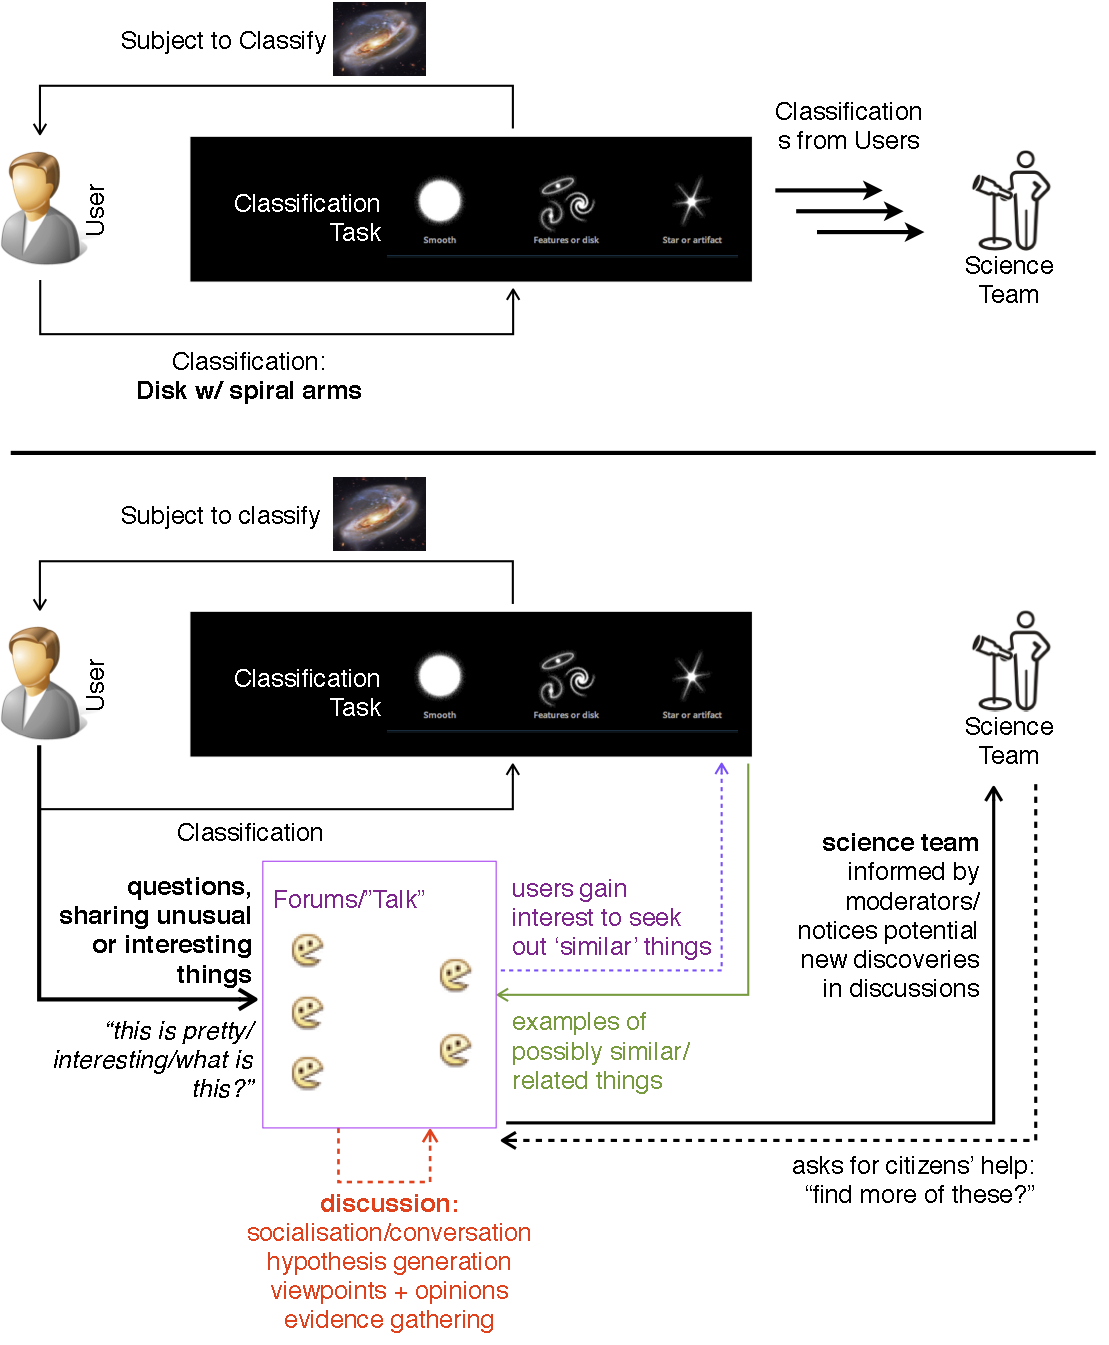
\includegraphics[width=0.44\textwidth]{imgs/twopaths.png}
\caption{\emph{Two paths to science} - In addition to the ``standard'' path (top) typical of human computation systems, where research questions are answered using annotations created by executing tasks, a second path, that of \emph{citizen-initiated serendipitous discovery} is illustrated on the bottom.  In this path, citizens initiate the process by pointing out or asking questions about subjects, spawning collaborative hypothesis generation in the discussion forums. Science teams, picking up on these discussion threads, then either perform a further investigation on their own, or start a collaborative investigation with the volunteers.}
\label{fig:twopaths}
\end{figure}


% Ultimately, this process sparked the discovery of several previously unknown species, planets and phenomena, that have proven thus far among Zooniverse's most significant findings.  Thus, the Zoonivese team see two major ``Paths to Science'', illustrated in Figure \ref{fig:twopaths}. We briefly describe four such phenomena here, highlighting the unique aspects of each discovery, and the roles of the individual parties in each.

\subsubsection{Individual Citizen-Initiated Discovery: \emph{Hanny's Voorwerp}}
In August of 2007, on the Galaxy Zoo forum, Hanny van Arkel, a Dutch school teacher who identified herself as user ``Hanny'', spotted an usual blue-shaped object in a subject beneath a galaxy, and posted a question in the Galaxy Zoo forum. Within an hour, two separate members of the science team had shown an interest in the subject and attempted to identify the shape, continuing to comment for a further thirteen days, concluding it was something ``weird [...] I\''d like to know what it is''. Thereafter, discussion on the thread stalled until December 2007, when Hanny asked about whether the mystery had yet been solved. The science team then redoubled their efforts to identify the shapes. After scientists made the thread more prominent, other Galaxy Zoo users began to post examples of other subjects, as well as collections of data, in order to help identify the shape. 

The object in question was not the main focus of the subject, which was in fact a galaxy located in the centre of the image. Since the classifying interface referred only to the galaxy, without the forum thread drawing attention to the oddity present, it is possible that it would have gone unnoticed. Hanny's thread did not result in significant contributions from users, but it was instrumental in drawing the attention of scientists to the object, allowing them to carry out further tests and analyses that users could not - Requesting for telescopes to be pointed at the object, for example. As a result, the discovery relied heavily on the science team but could not have taken place without the actions of an individual citizen. A more detailed chronicle of Hanny's discovery was documented by XX et al \cite{}.
%http://www.galaxyzooforum.org/index.php?topic=3802.0

\subsubsection{Group-Led Discovery: \emph{Galaxy Peas}}
Due to the technology used to capture the images used for Galaxy Zoo, subjects could appear in a variety of colours which did not reflect their colours in the visible spectrum. This resulted in objects appearing in subjects as green, when they are in fact blue. These green objects were particularly interesting to Galaxy Zoo users, who perceived green to be a strange colour for a galaxy.  The majority of such subjects simply included camera glitches, which had resulted in light only being absorbed in one filter, giving objects a green appearance. However, certain objects were not glitches and appeared as small, tight, green spheres. Users used the term “peas” to refer to the objects in question, after a joke thread started by the user ``Hanny'' on the Galaxy Zoo forums, 'Give Peas a Chance,' in July of 2007. The strange colour and shape of these galaxies captured the imagination of many galaxy zoo users, who formed a group called the 'Peas Corp' and went in search of subjects containing peas, creating various forum threads to collect them. While the science team were particularly busy in the early months, the collections of peas eventually drew their attention a year later in July of 2008 and they discovered that these galaxies shared  certain interesting features, including specific red shift values and bright spectral lines caused by double ionised oxygen particles (OIII). This resulted in a 'call for action' from the user ccardamone (a member of the science team) known as the 'peas project', which requested subjects containing peas with certain properties.

As a result of the peas project, users found and analysed various subjects in order to create a suitable list for further analysis. This allowed the science team to carry out various tests and statistical analyses on the objects, to attempt to explain the strange appearance of these particular objects and to identify what 'peas' are. This collaboration between the science team and the Galaxy Zoo user base resulted in a discovery which both sides may have missed otherwise: Users noticed the objects were strange, but did not realise their significance, while the science team were able to identify the significance, but may not have identified 'pea' galaxies as a specific class of galaxy, without the actions of the user base.

% http://www.galaxyzooforum.org/index.php?topic=3638.0 and http://www.galaxyzooforum.org/index.php?topic=270633.0

%comment from markus: consider adding the 'offline' communication stream here which happens when scientists start to discuss forum observations by mail for example. Is it possible to detect that something happened 'offline' by simply looking at what is visible online? How is the information flow between 'online' and 'offline' discourse? Are there specific actors delivering information into the one or the other direction? What about all other people which are not involved 'offline'? Do they know about this 'hidden' activity? Does it motivate or demotivate people when something is going on without them? Are all users equal in this regard?

% Hanny's Voorwerp is the clearest example of this - Evidently work is going on 'behind the scenes', but this doesn't seem to put users off - They don't seem to understand why they aren't allowed to know about things, but they do seem to wait somewhat patiently for the 'reveal' of information. However, it's quite possible comments which were more negative have been deleted or edited in the meantime and there's no way of knowing what was said by whom to whom outside of Zooniverse. Besides which, we can only tell that there's hidden activity when it's made somewhat clear - Which would be the same situation for users. Truly hidden activity would be just as hidden to us, at least from looking at the forums. In that particular case, the actors are Hanny and the science team - Moderators actively admit to not knowing anything.

\subsubsection{Asking for Help on a Possible Discovery: \emph{Convict Worm}}
In August (Potentially September) of 2012, the user 'illmarinen' made a comment on the talk page for a Seafloor Explorer subject, asking about an animal which was present in the image which he was unable to identify. A member of the science team responded, stating that she thought this could be a new discovery, which he nicknamed a 'convict worm', adding that he was actively seeking subjects where the worm was present. This resulted in a small number of users commenting on such subjects with the hashtag “convict-worm,” allowing scientists to easily collect examples of the potential new species. A blog post published shortly after the discovery encouraging users to tag convict worms has led to sustained and frequent tagging of subjects perceived to contain the worms, allowing suitable subjects to be gathered without requiring changes to the classifying interface, which did not allow flagging of convict worms.
%(http://talk.seafloorexplorer.org/discussions/DSF1002n2b?object\_id=ASF00009jp)

\subsubsection{In-Depth Citizen-driven Investigation: \emph{Kepler 16B}}
In May of 2011, Planet Hunters user Kian Jek made a comment on the Planet Hunters Talk website under the username ``kianjin", sharing a subject which appeared to show an eclipsing binary star with a third body present. A research team led by Slawson had already began analysing the system in question and it was eventually discovered that this system was a circumbinary system - A system in which a planet orbits two stars simultaneously. 

After the announcement of this discovery, named Kepler-16b, Meg Schwamb of the Planet Hunters science team published talk pages with links to all known eclipsing binaries present in the Planet Hunters data. In February of 2012, the user Robert Gagliano, using the username ``robert gagliano", searched through each of these subjects for signs of potential planets and noted two transit features (reductions in light intensity caused by a body 'transiting' between the star and the satellite) present in the subject SPH10052872. Kian Jek later predicted and confirmed a third transit and was then able to create models and graphs to better understand the lightcurves. Upon completing these models, Jek had confirmed to the best of his abilities that SPH10052872 showed a circumbinary planet and at this point, contacted the science team, who would be able to carry out further analysis which he could not. 

While Gagliano and Jek required the intervention of the science team to confirm their discovery, their research was much more in depth than in the other examples shown. Additionally, through their work, they had proven that something of interest was present and had successfully identified the item to the best of their abilities: They were not asking "what is this," but rather, they were asking for confirmation of their theories. 

% random comment to see if I'm still getting errors
\subsection{Towards More Effective Collaborative Discovery: \emph{Talk}}

%  original from Chris/Rob, turned into below
% It was designed to enable links to be made easily between classification and discussion and to allow science team members as well as advanced volunteers to quickly notice when users were talking about discoveries of potential interest. To understand the design drivers for talk's system of object-orientated discussion, consider the case of a new classifier who had spotted a `pea' in a Galaxy Zoo image. Even if they were to move to the forum, they would have been unable to search for discussion of their or similar objects unless they made the same mental leap to think of a small round celestial object as a kind of vegetable. If they found the right thread, they would have had to upload their image to a linear 	discussion which might well be in the middle of more detailed analysis. In Talk, by contrast, a single click after classification invites discussion, and lands on a page dedicated to discussing the object that's just been classified. Our putative pea-finder would immediately be able to see what had already been said about this system, and - were it already to be tagged as a 'pea' - to click on 'pea' and realize that there was a much broader conversation going on. This model has been broadly successful, with most of the discoveries made by the Planet Hunters project (including PH1b, the first planet in a system with four stars) coming from discussion between users who found interesting things in the interface and a community of more advanced workers who were able to help the science team follow-up on those discoveries. 

% ``number of emails received by the team'' -> what kind of emails? and how did this prompt use of a forum
%% Michael Nielsen's book > on networked science --- Reinventing discovery
%% http://press.princeton.edu/titles/9517.html

% Rob's original >> 
% Beyond achieving the goals set out to reduce this support burden, users made use of the site to identify, discuss and advocate for serendipitous discoveries. The canonical example is the object now known as Hanny's Voorwerp \cite{voorwerp}, a galaxy-scale glowing gas cloud which turned out to have been ionized by activity associated with neighboring galaxy's rapidly feeding black hole. In this case the discovery was reported on the forum, but the follow-up work was carried out by the science team themselves. In other examples, though, much more sophisticated behaviour was seen. The discovery of the Galaxy Zoo Peas \cite{Peas}, for example, saw a group of volunteers who had identified the presence of small, round and green objects (hence the name) in the background of some images work together to download and explore metadata on these objects, to write database queries and even, eventually, to create their own citizen science site to assist in further classification of these intriguing objects. The peas turned out to be a new class of galaxy, the most efficient stellar factories in the local Universe, and remain the subject of vigorous debate in the professional astronomical community.  The process by which the Galaxy Zoo science team picked up on the participants' posts in the Discussion forums about ``green peas'' and ended up with a significant new discovery is documented in detail on the Zooniverse Blog\cite{story-of-the-peas}.

%% specious stuff emax wrote, please check 

Over the course of the Zooniverse project, as the role of citizen discussion expanded from asking and answering questions to collaboration, it became clear that aspects of the design of the original forums impeded effective use for a number of different reasons.   

First, the forums used a standard linear message-board interface, comprising a set of top-level boards that each, itself, contained a set of message threads.  Each message thread, in turn, consisted of a linear sequence of posts; posts to a board either started a new thread, or were appended on the end of an existing thread.  Several drawbacks of this model became apparent as the board grew; first, threads on the same topic might appear in different boards.  Second, multiple threads on the same topic could appear within a board, which became increasingly an issue as the number of threads per board increased, and users found it increasingly difficult to identify relevant threads before creating a new one. (The main GalaxyZoo forum has several boards each with over 5000 threads that make up more than 100k posts, making navigation and retrospective analysis very daunting.)  Finally, since posts were strictly linked to a single thread, it was difficult for insights to be gathered on topics across threads; in particular, discussions about particular topics, such as types of celestial bodies, similar objects, artefacts, and phenomena would become fragmented among threads.  As threads grew in length (in discussions), topics often diverged from the topic of the top post, meaning it was difficult for users to anticipate the contents of a thread by looking at the thread's title.  

Given these forum limitations, it became the role of the forum moderators to monitor and de-fragment threads as necessary, moving posts between threads and even boards.  After trying to act as moderators themselves, the science team appointed a selection of the most active citizen participants with moderator privileges and status in the system.  But despite the dedication of this new group of volunteers, this proved often a challenging task as participation in the forums grew; the result was that regular members often posted messages to moderators to help them out, pointing out threads to merge and posts that would best fit elsewhere.

While this technique succeeded at the beginning, overall participation among new users (across all Zooniverse projects) levelled off after an initial period of growth, and many factors suggested that the difficulty of navigating the forums was responsible. Such low adoption rates among new users were seen across projects, although a small set of core contributors seemed to continue to use it regularly.  (In fact, this core community also resisted any attempts to modernise and migrate discussions to a more structured format, which we describe next).

 % and still is the mechanism by which the original Zooniverse forums operate today, primarily among a small set of core contributors.  overall participation levels in the forums levelled off after an initial period of fast growth. Such low participation rates were present across Zooniverse projects such as Moon Zoo and Old Weather, and messages suggested that it was the difficulty of navigating these forums that was its cause.  cross the boards, however, it is worth noting that a core community continued to use the forums with a space to discuss the historical aspects of the project, in particular.

%% key affordance: linking between subject and its discussion, and then horziontally allowing tagging as a mechanism of allowing similar posts to be identified

In response to these problems, the Zooniverse team decided to re-design the forums from scratch, departing from the linear messageboard structure.  Among the goals of this effort were to provide better integration with classification tasks, so that participants could more easily discuss subjects they saw directly and provide improved navigation capabilities that would reduce fragmentation witnessed among the forum boards and threads.  Starting from the launch of Planet Hunters in 2010, their first such system was launched, called \emph{Talk}.  

Talk offered several unique features; first, every subject had a unique \emph{talk page}, corresponding approximately to a thread where discussions about that particular subject could be centralized.  Talk pages were thus indexed (identified) by subject.  To support simple cross-referencing, Talk identified when the name or identifier of a particular subject was mentioned, and replaced the mention to the talk page of that subject.  

An additional navigational feature was added based on insights from the \emph{Peas} discovery above; in that situation, there was a need to be able to collect posts about ``green objects'' and ``objects that look like peas''.  To facilitate this, the team added hashtag-tagging support, so that tags added to a post could be easily collated with other Talk pages with the same tag.   This feature was used extensively during the ``Convict worm'' case described earlier; when the science team asked citizens to tag any worms matching their description with ``\#convict-worm'', this tag was quickly adopted by participants and generated a large number of hits of potential worms.  Allowing tagged-items to be viewed together and linked directly to subjects tagged by others successfully helped to channel participants who were previously unaware of the discussion to the collection of subjects and debate around them.

\subsubsection{Encouraging More Participants to Discuss}
%% TODO quant: any statitstics on discussion rate? 

Based on the discoveries described earlier, the science team began to perceive the tasks as serving a secondary important function beyond providing the labels and classifications as designed; namely, to serve as entry points to discussion, and show participants things they might want to discuss or talk about.   %In particular, this second function produces science through the intervention of `superusers' who may not classify themselves but who are able to make use of and further analyze interesting discoveries. observed that many of the comments provided some degree of insight and were useful when identifying unusual features of subjects.  
Unfortunately, however, it was observed that only a small proportion of users ever visited the discussion forums, and that those who kept the forum alive usually consisted of a small, core group of active participants and the occasional newcomer. Thus, to attract more diverse perspectives and to encourage more volunteers to contribute insight, the team sought to increase the proportion of volunteers who participated in the forums.

%    online communities \cite{lampe2010motivations}.  "power law distribution of participation" 

To do this, the team devised two strategies. The first was prompting users explicitly about whether they wanted to discuss an item after every task.  The goal of this was to get users who may have seen something interesting or ambiguous to think about posting about it, and second, to \emph{reduce the barrier to execution} \cite{norman2002design} to do so.  


This prompting was realised in a number of different ways; in Planet Hunters, the question 'Would you like to discuss this?' was asked after each task, increasing engagement with Talk at the cost of potentially slowing down classification work by adding an additional prompt in the main interface.  (The explicit prompts required as much effort to enter Talk as it was to dismiss the prompt - a single additional click.) As much of the Planet Hunters science has come from Talk, this trade seemed worth making for this project.  In the Milky Way Project,  meanwhile, launched a few weeks later, Talk was offered as one of three options after work on a particular subject is completed ('Save', 'Save and Discuss' - which leads to Talk, and Cancel).  This induced fewer participants to access the project's Talk features, which, in fact turned out to be the case, as visible in Figure \ref{}.  %% TODO quant


% TODO quant analysis : measure the effect of talk prompts >> 
% prompting people to use talk vs giving people the option to look at talk (among other things) vs ... 

\subsubsection{Avoiding Thread-Death}
% However, another significant factor influencing the success across instances of Talk seems to be involvement of the science team in discussions, especially in the first few days of a project. Early engagement allows trust to build up between moderators, community and professional scientists which sustains a community in the long term. This is now a key consideration in project selection and timing of launch. 

%% TODO reference :: authority thread death
The second strategy was devised to overcome the problem of \emph{authority thread death} \cite{} a problem frequently observed in online forums caused by a voice of perceived authority, usually either a moderator or merely confident person, posting in a forum, resulting in the thread being subsequently \emph{killed}, with no further participation.  The psychological explanations for authority thread death have been explained in terms of people not wishing to challenge authority, to there being a diminished need (e.g., since an authority has spoken, there is nothing further to be said).  Although killing threads seems to rarely be an actual intention of any of the Galaxy Zoo Forum moderators, as exhibited by their occasional efforts to try to revive these threads by asking rhetorical questions to seldom avail, this problem nonetheless occurred frequently in the original forum.

The second version of Talk sought to circumvent thread death by simply adding an additional affordance for adding a comment about a subject on the Talk page.  Taking inspiration from microblogging interfaces, the team decided to put a ``twitter-like'' 140-character box underneath each subject, to encourage participants to comment on the subject with whatever they liked.  This format, being less structured, formal, and more egalitarian than the forums, meant that people would only see a selection of recent ``tweets'' about the subject beneath theirs, and would be less likely to be put off by a moderator's input.  The status of each user, specifically whether or not they were a moderator or member of the science team, was also suppressed to reduce this effect.    

%% TODO someone: 
%% The effect of the introduction of this Twitter is ___________________________

\subsubsection{Active Collaboration with the Science Team}
Structured collaboration also proved effective. Galaxy Zoo science team member Bill Keel from the University of Alabama was able to spend time on the forum, and asked for help with searches for objects such as galaxies which appear to overlap \cite{overlap} (distant galaxies used to illuminate foreground ones can be used to probe the dust content of systems, a matter of some importance to astronomers). This work was also successful, but required Keel to spend substantial time as part of the forum community, something that other science team members were unwilling or unable to do. 

%% DOTO SOMETHING ELSE ABOUT COLLABORATION HERE?
%(This was perceived as not the only problem with the Forums and led to the design of the Talk forums, which anchored discussions around subjects, and reduced the need for a person, a role fulfilled Bill Keel to coordinate discussions about the same subjects or topics. and to make those discussions visible to both the science team and the participants.) Furthermore, by 2009 the forum had become less popular; the percentage of Galaxy Zoo users posting on what was a standard \emph{Simple Machines forum}\footnote{} was very low (less than two percent) and with more than 500,000 posts in more than 10,000 topics it had become difficult to navigate. While it still served the need of a core constituency, it was not engaging the majority of Galaxy Zoo classifiers in science. 

\subsection{The Forces of Engagement}

The second theme pertained to characterising the factors that drove user motivation and sustained engagement, specifically the aspects of a project  that attracted people to the project, motivated them to participate, and then maintained their interest over time. Here, we describe the key experiences and ways that these have impacted Zooniverse project designs.

\subsubsection{Interestingness, Implicit Reward, and Difficulty} 

Over the course of different projects, it became clear some projects experienced greater sustained participation and attention than others.  This led the team to enquire whether it was aspects of the task itself, data set, or domain that most influenced participants' interest and engagement within projects.  

%% TODO: XX AND YY here - please
This turned out to be a difficult question to answer.  However, through analysing forum discussions, in particular the reactions and focus of enthusiasm of forum users, the team derived several rules of thumb. Overall, the team concluded that, while there were many factors that influenced participation, three stood out; they were \emph{interesting-ness of subject}, \emph{difficulty of task}, and related to these two, the \emph{frequency and form of reward}.  These aspects seemingly eclipsed other factors, such as type of task, domain of origin, source of data.  The intrinsic ``interesting-ness'' of the subjects observed in some projects seemed to play a major in attracting and sustaining particiation.  By `interesting-ness' we mean subjects that involve viewing items that have aesthetic, fun, cute or emotional value, such as such as beautiful photos of galaxies, photos of flora and fauna (such as the candid photos of animals of Galaxy Zoo).  

Such interesting images only sustained participation if they appeared \emph{frequently enough}.  The team explained this by drawing from the theory of \emph{implicit reward} (e.g., \cite{implicitreward}); in the case of Zooniverse projects, no explicit reward was given for participating in a majority of the projects (except in Old Weather and Worm Watch Lab, where `points' of no monetary value were rewarded for completing tasks).  Therefore, for most of Zooniverse, rewards remained purely implicit in the tasks they were given next.  Therefore, when such new tasks involved viewing subjects that were occasionally very beautiful, interesting, or at the very least \emph{variable}, participants were driven to keep looking.  Since Zooniverse intentionally provided no \emph{skip} facility, viewing more subjects required completing more tasks.

In the first launch of YYY, participation dropped off because the frequency of reward was simply too low; a participant could be made to look at more than 1000 blank subjects before coming across one that contained a Galaxy! 

\emph{Facility and speed} with which tasks could be executed seemed to provide a different kind of reward feedback that spurred sustained participation; projects with tasks that were quick and easy generally continued to be used for a longer total duration than those that had more complex individual steps that required careful analysis or complexity.  This effect was found to be so strong that the team found this often trumped \emph{interestingness} altogether; people were willing to slog through thousands of photos of boulders in \emph{Moon Zoo} despite them all looking basically identical with little hope of any further reward or variation because each task was quick and easy to do.  Participants performed an average of $MMM$ classifications of Moon Zoo, compared to $YYY$ comparable tasks, for example in ZZZ, a substantially more difficult project.

% TODO:
% Galaxy Zoo Craters vs Milky Way Project Bubbles - Essentially same task, but Bubbles much more complex due to arc tools - fill in MMM, YYY and ZZZ above with figures from these projects. Note that from March 8th 2012, the Milky Way Project changed to only include subjects which were guaranteed to contain a bubble - seemingly, no change has been made to the interface itself.

By comparison, there was no perceived preference in research field, topic, or task type, and substantial variability among the success rates for projects existed within each of these categories.  For example, astronomy projects such as XX maintained attention and engagement, while YY, also from the same field and of essentially the same task type, levelled off in participation after an initial period of enthusiasm.   Furthermore, it was deemed that tasks of one particular type, such as classifying tasks, were not significantly more successful than transcription, given the success of projects like \emph{Old Weather} and \emph{Notes from Nature}, although the very different nature of these tasks makes direct comparison difficult.

% that appealed to the general audience, and it was these projects that exhibited the greatest user retention as well as attracted the most users.  In particular, Galaxy Zoo, which features a large number of beautiful photos of galaxies and deep space, and Snapshot Serengeti, which features an abundance of ``candid'' photos of popular animals in the wild were each 

\begin{table*}
\begin{center}
\small
\begin{tabular}{lllp{1.1cm}p{1.1cm}p{1.4cm}p{1.2cm}p{1.4cm}p{2.5cm}}
\hline
Project & Classifications & Favourites & Avg Favs per classif. & Favourite workflow & Talk items & Avg talk per classif. & Talk items per Subject & Talk workflow \\
\hline
\hline
Ancient Lives & ??? & ??? & ??? & ad hoc & ??? & ??? & & ad hoc \\
Andromeda Project & 1,091,406 & 5,874 & 0.005 & prompted & ??? & ??? & & prompted  \\
Cyclone Center & 218,317 & 1151 & 0.005 & prompted & 1615 & 0.7\% & & prompted \\
Galaxy Zoo 2 & 7,907,151 & 218,405 & 0.028 & ad hoc & 89,956??? & 1.1\% & & prompted  \\
Galaxy Zoo Hubble & 7,458,781 & 214,101 & 0.029 & ad hoc & ??? & & & prompted  \\
Milky Way (Bubbles) & ??? & ??? & ??? & none & ??? & ??? & & prompted \\
Milky Way (Clouds) & ??? & ??? & ??? & ad hoc & ??? & ??? & & ad hoc \\
Notes from Nature (Herbarium \& Calbug) & 209,169 ?? & - & - & none & 4,208 ?? & 2.0\% & & ad hoc \\
Notes from Nature (Ornithological) & ?? & - & - & none & ?? & 2.0\% & & prompted\\
Planet Four & 3,900,785 & 40,657 & 0.010 & ad hoc & 32,097 & 0.8\% & & prompted \\
Planet Hunters & 19,179,696 & 201,508 & 0.011 & ad hoc & 427,917 & 2.3\% & & prompted  \\
Seafloor Explorer & ??? & ??? & ??? & prompted & ??? & ??? & & prompted \\
Snapshot Serengeti & 7,800,896 & 116,758 & 0.015 & ad hoc & 39,250 & 0.5\% & & prompted  \\
Space Warps & 7,037,472 & 34,977 & 0.005 & ad hoc & 20,978 & 0.2\% & & ad hoc \\
Worm Watch Lab & 90,350 & 438 & 0.005 & prompted  & 855 & 0.9\% & & prompted  \\
\hline
\end{tabular}
\caption{\emph{Favourites and Talk Items per Classification per Project} - The above table shows the number of favourited relationships and talk items in the Zooniverse database as of September 2013, for each of the above the projects.  (Only projects that used Zooniverse Talk were included to allow direct comparison, and Galaxy Zoo Forum figures were not included, which can be found directly on the forum site.) In the ``workflow'' column, ``prompted'' means users were prompted with a dialog asking whether they wished to discuss the item, while ``ad hoc'' means a button providing access to the talk page for that subject was made available in the interface for users at any point.}
\label{tbl:favourites}
\normalsize
\end{center}
\end{table*}

% time periods: Galaxy Zoo 2 (2009-02-16 - 2009-05-21), Galaxy Zoo Hubble (2010-04-17 - 2012-01-31), Planet Hunters (2010-12-15 - 2013-07-16), Cyclone Center (2012-09-27 - 2013-06-12), Andromeda Project (2012-12-04 - 2013-07-17), Snapshot Serengeti (2012-12-11 - 2013-07-17), Planet Four (2013-01-07 - 2013-07-17), Notes from Nature (2013-04-19 - 2013-07-17), Space Warps (2013-05-07 - 2013-07-17), Space Warps (2013-05-07 - 2013-07-17), Worm Watch Lab (2013-07-03 - 2013-07-17)

% Based upon popularity of the various projects and tasks, the team gained considerable insights on the tricky question of \emph{what drives people to keep coming (back)}.   
% Tasks, however that were not particularly interesting can still sustain engeagement if they are \emph{easy}

% Since Galaxy Zoo 2 there have been project-o-meters' created to show progress of the community toward a common goal or project completion. The Planet Hunters `Planetometer' displays the total number of classifications of the project, as well as the number planet candidates discovered. The `Moonometer' shows the cumulative area of the Moon that Moon Zoo has scoured for craters in various units\footnote{Units include Square Miles, Football Fields, Taj Mahals, Switzerlands, Utahs, Texas, Polands, Wales, Whales and others -- see http://www.moonzoo.org/moonometer}. These counters exist on many projects but not all.

% Where they do exist these counters do not normally appear to drive people to participate, but they do appear to be heavily discussed by people writing about projects and by dedicated users noticing the approach of milestones. In the case of Galaxy Zoo 2 there was a drive toward 60 million classifications in March 2010, to mark the completion of the project; whereas in Old Weather the imminent arrival of `100\% Complete' on the homepage caused users to slowdown and literally ration themselves to abate the project's conclusion.

% Individual counters of a single user's classifications have existed for several projects as well as result in people talking about their own classification count. A volunteer's counter for all projects has existed on the the Zooniverse homepage\footnote{http://www.zooniverse.org} for two years but is rarely discussed and in fact many regular users of the site have no idea it is there!

% More recent Zooniverse projects have been able to include synthetic or expert data. This has meant that in many cases a user can be given instant feedback on their classification. Reactions have been almost universally positive, and it appears to give confidence to some users who might otherwise have not continued with the project. The most recent example is Spacewarps, which gives continuous feedback, although at an ever-decreasing rate, throughout a user's time on the site.

\subsubsection{Tutorials: Harnessing One-Hit Wonders}
A common challenge to many human-computation systems is in teaching new users  enough about the tasks being asked of them for them to be able to carry them out effectively.   One common approach to getting users familiarised with a task or set of tasks is to brief them with a \emph{tutorial} of some form, when introduced to a new class of tasks \cite{gutheim2012fantasktic}.  However, designing an effective tutorial requires addressing a multitude of design questions, such as whether the tutorial should be interactive, or simply explanatory text or video? How much background about the task should the tutorial go into?   How long and thorough should the tutorial be?

In citizen science, these questions are particularly difficult to answer because of the specialised nature of many of the tasks.  Some of the classifying tasks of GalaxyZoo, for example, involve identifying properties of intergalactic phenomena that most users may not have even heard of prior to participating.  Similarly, even more ``down to earth'' domains such as Snapshot Serengeti involve identifying animals among a huge variety of species, many peculiar to the Serengeti habitat, such as the \emph{secretary bird} or \emph{aardwolf}. How are users to possibly know how to identify and classify creatures and phenomena they know nothing about?

A second consideration was tied to the intrinsic motivation factors discussed earlier; since users were motivated by their own curiousity and desire to help, if users were taught more about \emph{what} they were looking at, or the purpose of the scientific investigation, then would they have become more likely to contribute?

The team struggled with these questions and designed a variety of different kind of tutorial resources during the project's trajectory.  This gave considerable insight to the tutorial process, including the kinds of factors that matter the most and design guidelines for successful projects.

% The first, the team could not emphasise enough; by letting new users immediately start contribute the moment they access a project site, they not only feel like they are instantly contributing, but this can be harnessed as useful work in the likelihood that they \emph{never come back again}.  (This was perceived as particularly important because, regardless project attractiveness, the number of so called ``one hit wonders'' is likely to vastly outnumber the number of returning users.)  

In short, the result of this investigation was \emph{get users involved immediately}, and \emph{open up paths to learn more}.  This first observation was derived from several specific experiences pertaining to designing interactive and video tutorials; neither were very successful, dramatically reducing the number of people who made it to the first task.  For example, when a new mandatory tutorial was designed and introduced in Moon Zoo in respose to questions in the discussion forum, the number of new users dropped from XX-YY to 0.5 per day.  Making users watch an introductory video had a similar effect.

The implication of this observation was the need to devise an interface which could get new users on a real task immediately, without any introductory explanation.  This necessitated some way for new users to understand what to do; the team opted to build such guidance into the task interface itself where possible.  For example, in Snapshot Serengeti the team provided multiple \emph{interaction paths} within a single interface in order to support both new and experienced users; while new users could address a sequence of step-by-step questions such as ``Looks like (a horse)?'' that each narrowed down a set of possible animal species based on attributes as in a decision-tree, advanced users who could identify the animal could directly select the relevant species from a matrix to the right (see Figure \ref{fig:snapshot}).

The only problem with this approach was that there was no feedback to users about how well they were doing.  Since feedback is necessary for improving a skill, the team selectively introduced, at a pre-deteremined frequency ``gold standard''  tutorial tasks on several projects, including Planet Hunters, the Andromeda Project, and Space Warps, that looked just like normal tasks, but were created by hand.  If the user failed to achieve the correct classification on these gold standard tasks, guidance in the form of a small explanations of the correct answer(s) were provided.   

The effect of the combination of these design decisions had a measureable impact on the amount of information that the Zooniverse project has managed to successfully elicit from users.  The team estimates that a net $Y$ percent of classifications made in the system were yielded from one-time users that never returned.  This number would have been greatly diminished if the traditional approach of putting users through a tutorial process at the beginning of the tasks had been taken instead.

% the strategy is to  letting users use help affordances to get more information about what to do or clarifications regarding terminology.  For example, on Planet Hunters, users are shown a real subject () immediately and asked questions about whether it has any \emph{transients}.

%The key lesson gained through this experience was, to be put succinctly, participants need to be able to contribute from the first moment they are set upon a task.  Any attempts to occupy participants with mandatory tutorials or tutorial videos will ultimately dissuade participation, resulting in a loss  of a potential contributor.  

% How does one then allow people to perform a task when 

% The key tehThe key themes were that \emph{tutorial videos don't work}, \emph{mandatory interactive tutorials annihilate participation}, and \emph{getting people to contribute }.

% Citizen science is no exception to this, especially as many kinds of tasks benefit from appropriate domain knowledge about the subject.  For example, knowledge about how intergalactic bubbles and clouds typically appear, vary in appearance, and how they are formed could help an individual identify them in their respective stages of development. 
% brings one into conflict with several other requirements. In particular, Zooniverse projects are designed to get useful classifications from those who only visit once; an overly elaborate or time consuming tutorial leads to these casual visitors leaving without ever having done anything `real'. This is problematic not only in terms of lost effort but also in failing to present an authentic experience of participation, the very thing that seems to engage potential citizen scientists to return. Tutorial design, therefore, has tended to emphasize presenting only the 

% The original Galaxy Zoo included only a few lines of tutorial, followed by a simple test (as described in \cite{Lintott}). The aim of this was both to ensure a minimum level of classification accuracy and to provide feedback to users who it was felt might need reassurance that they were on the right track. However, to encourage participation the bar was set extremely low and the test was essentially ineffective; classification accuracy was ensured by later data reduction, a pattern followed by subsequent projects. Galaxy Zoo 2 included a longer, optional, tutorial which few users read, leading to the adoption (by, for example, Moon Zoo) of video tutorials which no-one watched. The solution now adopted was an inline tutorial which guides users through the interface quickly and gives feedback on classification of one or more initial subjects.

% This solves the problem of teaching classifiers what is expected of them, but consistent learning takes place throughout a citizen scientists' career. \cite{Smith}, for example, shows trajectories of classification accuracy for individual users, showing that while large changes most often come early in a user's encounter with a project dramatic changes in accuracy are possible throughout. Each classification provided by a user produces a (perhaps unknown) change in user behaviour through learning, information about the subject under classification and information about the user themselves. Projects such as Planet Hunters, the Andromeda Project and Space Warps include expert-classified or synthetic data which can be used to measure user performance. When presented with synthetic data feedback is given to the user on their performance - essential in preventing them getting excited about discovering simulated planets but which also forms as an ongoing tutorial. 

% Video tutorials don't work. People do them but then leave (Solar Storm Watch). %% TODO: Quant - can we show a graph of this?
% Compulsory training results in a large bounce rate (Moon Zoo) %% TODO: Quant - can we show a graph of this too?
% With Whale FM and Ancient Lives we used tutorials that were interactive and overlaid on the interface - seemed to work well.
% Then we moved on to the next logical step, which is guiding a user through a classification by annotating the interface as they go along. That's where we are now. % - Snapshot Serengeti is a good example of this 

\subsubsection{Avoiding the \emph{Don't Know} Escape Path}
A common complaint from the beginning of Zooniverse among participants in online forums was a lack of an \emph{I don't know} or \emph{Skip to next} button.  The omission of such a button was a deliberate design decision among the Zooniverse team, and, as discussed in a FAQ of the Zooniverse forum by the Zooniverse team lead, ended up serving additional benefits beyond those that were originally anticipated \cite{afron-blog-post}.

In particular, not having a \emph{Don't Know} button meant that individuals were required to perform a task in order to see more subjects; as described above, the  potential ``luck of the draw'' of receiving an interesting subject with their next task was a significant motivator for keeping people involved in the classification project.   (Had there been a ``don't know'' button, then this could have been used to quickly game the system and zip through subjects to find those of interest, thereby decreasing motivation to do the tasks).

A second result is that it forced users to slow down.  This is often  particularly valuable to the science team, as these particular \emph{hard cases} can yield clues that benefit most from human insight and problem-solving skills, and that allow systems to tackle subjects that are particularly difficult to automatically process - examples of which existed throughout the projects.  For example, subjects from the Snapshot Serengeti project were captured by motion-sensitive camera-traps triggered automatically.  Various situations, such as the camera being triggered simply by strong winds, animals brushing up close to the camera, or motion detected at night, meant that there were often images in which no animal was visible, only part of an animal was visible, or the subject was too close, out of focus, or mostly obscured. 

However, even in challenging cases, valuable partial information could often be obtained by pooling the collective judgements of individuals.  For example, if there is significant agreement that the animal visible in an image is large, the science team can use this knowledge as metadata to later retrieve the subject when doing a query for large mammals, such as wildebeests. Thus, even if the exact identify of the animals is unknown partial information can be useful to the process.  % Figure X displays an example of collective disambiguation process for a subject with a partially obscured creature. As can be seen, X Y and Z..

% Table here? May require slight rewrite of above text 

The other case is that not having a \emph{don't know} button coupled with the existence of a ``discuss'' button channeled individuals to talk about and collaboratively disambiguate difficult cases.  Examples of such collective sensemaking abound across the projects, especially for classification tasks where users routinely trade insights on what they think a particular creature might be and why.  

% the science team can be relatively certain that the animal in question is large and so not of interest when they are studying smaller animals. Alternatively, it may still be possible to identify what the animal is actually doing (eating, moving or interacting, for example) even if the identity of the animal is unknown. 
%However, such classifications can still be of value to the science team. Since multiple users classify the same subject, similarities between the classifications can offer valuable clues to the identify of the animal in question. 

% For particularly difficult images, the absence of an \emph{I don't know} button is particularly advantageous. Since multiple users are able to classify the same image, the team can identify similarities in responses. The modal response, for example, may clearly identify animals in the subject, or allow a more confident classification to be easily made. Additionally, this prevents an absence of classifications for more difficult subjects, which in turn allows the team to reduce the proportion of difficult subjects which each user is shown; If the system requires a specific number of responses for each subject, then the more a user skips a subject, the more unique users that will see that subject.

% HELP NEAL

\subsubsection{Value of Context and Narrative}
%% Old Weather stuff here
Sometimes the original source of data in a citizen science experiment can provide context that engages users and drives participation.  Here we describe the case of \emph{Old Weather}, a project that was originally scoped to get citizens to transcribe weather logs from old ship logs, but which has blossomed into a community of citizen-historians and other users interested in maritime history. 

The purpose of Old Weather, introduced in the Background section, was to use meteorological readings taken by sea captains of 19th and 20th century ships to build long-term models of ocean climate. However, many of the ship logbook pages where these measurements were methodically taken also interleaved other information about procedures and events taking place on the ship, such as crew and cargo movements, maintenance procedures, and so on.  Alongside many of these logs, there were occasionally random other things, including draft letters home from ship members.  Initially, the team intended to prevent users from seeing this additional information which were irrelevant to the weather transcription task, and of no interest to the science team. However, segmenting this additional information out was difficult to do automatically, and a task in itself.  Therefore, it was decided to leave the pages intact, with the hopes that it might add interesting context while not distracting from the primary task. 

However, this ``additional info'' was embraced by participants as clues to a partially-obscured history, and discussions blossomed on the forums about the significance of particular letters and activities on the ship.  Participants exchanged thoughts on who the recipients of the letters may have been, the meanings of particular terminology (e.g. ``holy stone?''\footnote{Old Weather Forums - \url{forum.oldweather.org/index.php?topic=3144.0}}) and discussed the history of each of the ships and the crew members on board.  Participants brought to the discussion information in from diverse historical sources both on and offline.  While this kind of participation may have not directly benefited the transcription task, it drove significant attention to the logs, and patched together interesting segments of a narrative history that may have not been otherwise given attention.  %The science team to allow some of this informal knowledge to be captured during transcription, by adding an ``events'' column to which users were encouraged to add ``any information which interests them.''  Historians are now consulting these logs to see if any new insight can be derived from the detailed events transcribed by these participants.

In retrospect, the design of the \emph{Old Weather} interface fostered this growth in several ways; first, an early decision to organise ship logs by ship, ship route, and chronology allowed users to easily identify logs by the same crew and route. (Other zooniverse projects, in contrast, displayed subjects typically based on which ones needed annotation, and displayed them to with little or no user-discernible ordering). Thus, preserving the context and provenance of information was seen to be sometimes extremely effective towards engaging interest from a wide and variet participant community.

% The result of this 
% The project interface only allows users to transcribe information pertaining to certain topics, such as date, location and weather observations. There is an additional ``events'' column to which users are encouraged to add ``any information which interests them.''
% Above "any information which interests them" quotation taken from Old Weather project FAQ page: http://www.oldweather.org/faq
% The additional information provided for the Old Weather project has not only helped attract users to the project, but has offered valuable data in its own right. Not only have the additional details provided a significant talking point for those using the project's forum, but also these additional details have provided a rich subject of study for various amateur and professional historians. By adding narratives and context to the data, the system has allowed users to engage with the project in a way that would have otherwise been impossible, not only through the classification system, but also through the discussion forum.

%% TODO TODO >>>>>  This needs to be fleshed out 
% \subsubsection{Socialisation and Sharing}
% %% Ramine/Neal others: is there anything we can say here?

% % The nature of the subjects used within the Snapshot Serengeti project, as candid images of exotic animals, has resulted in the subjects proving very popular - In August 2013, the science team submitted 12 images to the BBC's Camera-trap Photo of the Year competition, based upon recommendations by users. 
% The ``power of the crowd" to share and socialise has played an instrumental role for the Snapshot Serengeti project. When the project was denied further funding and facing closure, the science team turned to the Snapshot Serengeti user base for help. Realising that the nature of the subjects used for the project made them suitable material for sharing, the team encouraged users to turn the subjects into memes, which could then be shared to draw in new users. The campaign aimed to encourage new users to the site, who would see that the project was in financial difficulty and donate, so that the project could continue.

% In order to facilitate the sharing of objects, a ``meme this" button was added to the talk page for each subject, which allowed text to easily be added to the image. 

\subsubsection{Other factors: Design/aesthetics, Devices and Media}

%% \emph{This area under construction by emax}
%% Examples of surface level/aesthetic re-design >  (and perceived effects)
%% MoonZoo : redesigned December 2011 - re-designed the web site around the interface, interface had a slight modifications, and perceived effect? 
%% TODO quant: can we see any effect? look to see if there was any effect? >> not as far as we can see

% Does good design improve participation?  Much evidence has suggested that \emph{good design builds trust}, by improving people's subjective appraisal of web sites and applications.  However, there was no visible effect on the measures used to assess per-participant engagement on the site before and after the re-design of MoonZoo

It is well established in the web design industry that a well-designed website or application creates trust in new users and comfort among returning visitors, e.g. that ``good design builds trust'' \cite{someone}.  Moreover, rising standards of visual and interaction design across the Web have driven rising expectations in design standards from all web sites.  Given these observations, the Zooniverse team sought to ensure their projects met a high standard of design.  But how much design is \emph{enough} for an often budget-limited citizen science project?  

Starting in 2010, the Zooniverse team expanded to hire a team of professional designers, beginning with the Old Weather, Milky Way, and Planet Hunters projects to seek the answer to this question.  This team was also responsible for the re-design of Galaxy Zoo between its first and second launch.  Based on these experiences, the team remain convinced that although the strong design aspect of Zooniverse projects have become a hallmark of Zooniverse as a whole, they failed to observe any direct, impact on re-designing the interface on participation or engagement.  

\emph{Ice Hunters}, in particular, proved a valuable example in this regard; this was a project that was widely derided for its design in the discussion forums, yet remained very popular and achieved $XXX,YYY$ classifications.  This was taken to be an indication that factors pertaining to the subjects and task difficulty (for which Ice Hunters sat at the ``easy'' and ``clear'' end of the spectrum) may be more important towards sustaining participation and than aspects of visual design and interface layout.

\emph{Other interface trends} - 
In 2012 and 2013, there has been a rising fraction of users accessing Zooniverse sites via iPads\footnote{Interestingly, there were exceedingly few Zooniverse users who used non-Apple tablet computers.}. This led the Zooniverse team to usability-test the tasks and dedicate a development effort towards ensuring that these tasks could be performed using the various iPad screen sizes and resolutions that these devices offered. 

The team also looked at the impact of primary interface modality on project popularity.  In particular, it was noticed that projects that involved use of audio classification, namely \emph{Whale.Fm} and \emph{Bat Detective}, both failed to sustain as much attention as those that relied on visual elements.  The team is planning on investigating possible reasons for this disparity in the future.

% \subsection{Launching and Outreach}


\subsection{Launching Projects}

\begin{figure}[tbp]
\centering
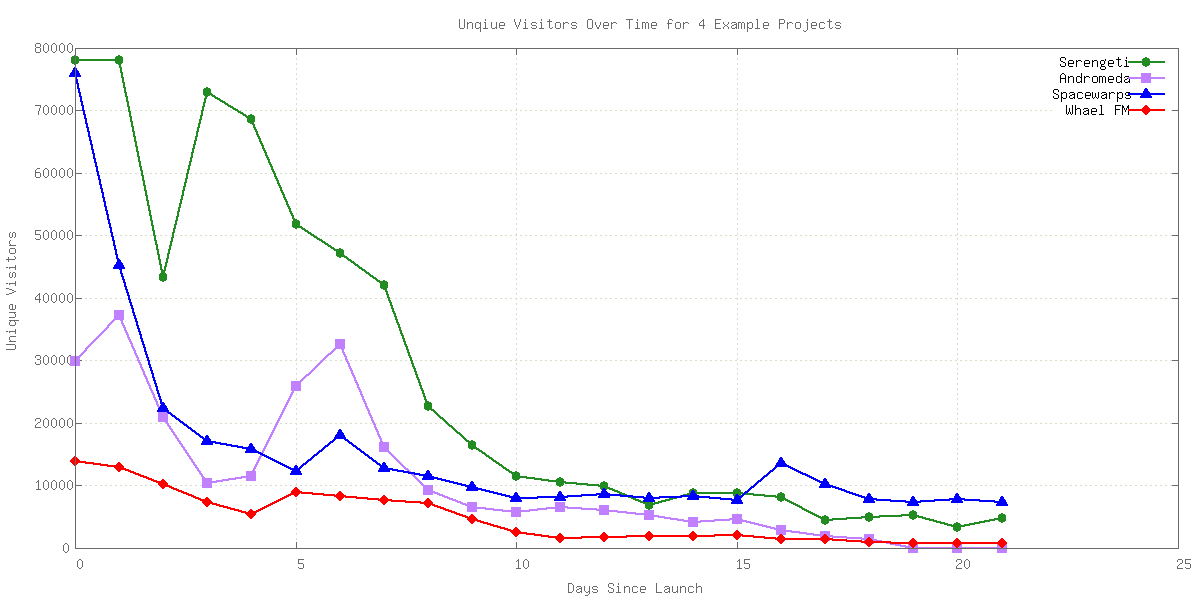
\includegraphics[width=0.50\textwidth]{data/launch-profiles/launch-profiles.png}
\caption{\emph{Launch profiles for 4 example Zooniverse projects} - Displays the number of users per day for the first three weeks of four projects: Snapshot Serengeti, Andromeda Project, Space Warps, and Whale FM}
\label{launchprofiles}
\end{figure}

% Andromeda, Whale FM, Spacewarps and Snapshot Serengeti as case studies

The final theme we discuss here pertains to launching projects and outreach efforts, including the use of social media, newsletters, and other promotional material.

It is a common misconception that websites are busy by default. Significant publicity and attention are often required to reach the right potential audiences for an online citizen science project. Networks and communities exist online to allow people to discover and share online projects, and are a valuable starting point for finding such individuals. The Zooniverse was one of the first organisations in this field and has grown a substantial network of people around it (\~860,000 at time of writing).

Shown above in Figure \ref{launchprofiles} shows the number of users per day for the first three weeks of activity on four Zooniverse projects: Whale FM (Nov 2011), The Andromeda Project (Dec 2012), Snapshot Serengeti (Dec 2012) and Spacewarps (May 2013). Each project displays a subtly different profile of activity in its first days and weeks. Snapshot Serengeti and Space Warps enjoyed a healthy start of 80,000 users on launch day, mostly consisting of existing Zooniverse users (from other projects) responding to the launch announcement newsletter. % For example ... X and Y .... 

As can be inferred from this, Zooniverse projects draw a substantial number of contributors from the pre-existing greater Zooniverse community. The Andromeda Project, mentioned above, was completed in a mere sixteen days thanks to a surge of activity from existing Zooniverse members, meaning all subjects were classified and tasks completed fully during this period.  Without this community, would have taken much longer.  Similarly, the initial surge in traffic on the Spacewarps project had 10,000 people contributing 500,000 classifications in its first twenty-four hours, and continued to sustain participation, with more than 10,000 people unique visitors daily even three weeks later, a majority of whom were seasoned ``Zooites''.  By comparison, it took weeks for blogs and news sites to pick up on the project and publish about it more widely.

Thus, while a substantial quantity of useful work can be done by one-time visitors described earlier, having a core community propelled many of the later project launches, bringing quick attention and results faster than any normal recruitment mechanisms would have.  

Zooniverse was not without its coverage in major media outlets, however, with the team benefiting from coverage in both traditional media outlets and online media, including international media networks such as the BBC (on \emph{The Sky At Night} and \emph{Click}), widely-read scientific magazines including regular coverage in the ``Citizen Science''` column of \emph{Scientific American}, and featured articles in \emph{National Geographic} \cite{zooniverse-natgeo}.  Such coverage regularly resulted in traffic spikes and influxes of new users.

Beyond publicity, the Zooniverse team identified several factors that influence parcitipation at launch.  First, having a `Call to Action' appeared to improve retention; moreover, sites with less text, and clear, succinct front-page messages descriptions of a project had lower bounce rates overall.  This was first seen clearly with Planet Hunters but also with Galaxy Zoo's fourth incarnation. 

% However above simple awareness, any creator of a citizen science project should be aware of the approximate effort required. Most Zooniverse sites enlist the help of tens of thousands of online volunteers. Thus when projects are designed, consideration should be given to the scale of the endeavour being attempted. Taking into account a reasonable expectation of web traffic and the effort any person may put in is difficult (how long is a piece of string?) but important for establishing a project with a realistic end goal within the required time. Simply producing a citizen science website does not guarantee popularity -- or more importantly scientific completion of the intended task.

% Difficult to form community without 'luck' - Sky at Night and media plugs for various projects, for example, more down to who is on the team. Certainly not users flocking to Zooniverse just because it exists.

% With more than 27 projects launched over just a few years, the Zooniverse platform is host to a series of natural experiments regarding the announcement and subsequent take-up of citizen science projects. There are a large number of variables affecting the potential uptake of any new site including but not limited to; method of announcement (e.g level of press coverage, size of existing community), `stickiness' of proposition (i.e. discovering an exoplanet is generally more exciting as a proposition than differentiating genetic subsamples of nematode worms); difficulty of task; technological requirements (e.g. Does the site work on desktops, tablets, smartphones); and many more.

% TODO: Rob - Add annotations to this plot and talk about events that influenced the profiles. Note that the launch iof Serengeti gives Andromed a boost a week in.
%Add annotations to this plot and talk about events that influenced the profiles. Note that the launch iof Serengeti gives Andromed a boost a week in.

% \subsubsection{Response from Existing Zooniverse Community}

% After the launch of each project, the entire Zooniverse community is emailed an announcement with an explanation of the new project, and how to participate. This pre-existing set of users -- who already have a sign-in for any new Zooniverse site -- is often enough to create a sizeable surge in activity in the early days of a project. In cases where no press coverage exists, this initial boost is sometimes crucial in producing useful data. The case of the Andromeda Project is particularly interesting, as this was the Zooniverse's first new space-based project for almost a year and it did not receive significant press coverage. However, the response from the Zooniverse community was so large that it completed its entire requirement of 1.1 million classifications in sixteen days. Similarly, the initial surge in traffic on the Spacewarps project was impressive (10,000 people contributed 500,000 classifications in its first twenty-four hours) and sustained (more than 10,000 people were visiting the site every day even three weeks later), and it took days for blogs and news sites to pick up the project and publish about it more widely.




% TODO: Can we show a visual example of a call to action versus not?


% http://blog.andromedaproject.org/2013/01/14/first-results-at-aas/ is the source for the change above from "just over two weeks" -> 16 days

% \subsection{Sustaining Engagement}
% Consistent with visitation patterns to most web sites \cite{TODO}, it was observed that visitors to the Zooniverse apps were increasingly likely to leave the site every passing minute on the site, than to stay.  Moreover, since after a user left, the probability that they would ever return was estimated to be at most an odds ratio of $10-to-1$, maximizing the amount of participation meant engaging users with tasks as soon as they first landed.  This had profound implications on the design of the tutorial, as we describe later, getting users acquainted to the system and their task.  The result of optimising this process, however, did allow a significant amount of contributions to be gathered by short-stayers; ultimately, over half of Zooniverse's classifications were performed by users who only visited the site \emph{once}.

%% immediately was a priority for maximizing the amount of potential participation overall.  Even more the likelihood of a later return to the site was (Over half of the classifications were contributed by users who never returned. This of course, has significant implications 
%% From the very first moment that a user arrives on a website, they are more likely to leave than to stay. The faster they can be engaged with participation in the main (citizen science) task, the more people will have participated over all.
%% % TODO this has a significant implication for the training/tutorial phase for getting new users oriented with their task, as users are likely to leave

% \subsection{Engagement: Interestingness x Difficulty x Context}
% By no surprise, a key factor that sustains participant motivation pertains to interesting-ness of the subjects themselves.  For example, those who witness ``beautiful'' galaxies in Galaxy Zoo, or an image containing interesting animals in Snapshot Serengeti, will stay longer and perform more classifications than those who did not see said images. In the case of projects where the subjects may not be inherently interesting, such as Old Weather, use of additional information and context can increase how interesting a subject is to users. In Old Weather, this included log book pages which were not related to weather data, which have resulted in significant numbers of discussions through the project forum.
% To measure the importance of the inherent interest a subject holds for engagement, we identified which subjects were most favourited, and examined whether those users who witnessed these subjects stayed longer, which was significant (Statistical measure). %TODO: Rob please!

% % Another key factor seems to be the graspability of the task - (and this can be challenging; for example, Galaxy Zoo is not about discovering galaxies, but documenting galaxy evolution as a function of their geometry) 

% A third factor pertains to task difficulty. Projects with innately simple to perform tasks (e.g. Ice Hunters, Spacewarps) show much higher classifications-per-user numbers than projects with more difficult tasks (e.g. Milky Way Project, Cyclone Center). The complexity or difficulty of a task does not appear to be correlated with how long users spend on the site in any session, however; Moon Zoo and the Milky Way Project have similar interfaces but very different dwell times. Conversely, Ice Hunters and Old Weather had similar dwell times for many months, despite one being far more complex than the other.

% % Having a clear call-to-action / message
% % Feedback: progress TODO: (move up here from down below)

% %%   % TODO: can we say anything about the effect of the narrative in Old Weather? 
% %%   % evidence in the discussion forums ? 
% %%   %   > i wonder why the handwriting has changed?
% %%   %   > most keen to help each other out -- 

% %% did they create rules - placing limitations to achieving the goal -> make a challenge
% %% what feedback system did they use and what was the overall goal
% %% icebergs/seal hunting : people really wanted a seal. :( 
% %% audio :: 
% %% posters vs 
% %% adding context: old weather
% %% achieving flow state

% Since Galaxy Zoo 2 there have been occasional project-`ometers' created to show progress of the community toward a common goal or project completion. The Planet Hunters `Planetometer' displays the total number of classifications of the project, as well as the number planet candidates discovered. The `Moonometer' shows the cumulative area of the Moon that Moon Zoo has scoured for craters in various units\footnote{Units include Square Miles, Football Fields, Taj Mahals, Switzerlands, Utahs, Texas, Polands, Wales, Whales and others -- see http://www.moonzoo.org/moonometer}. These counters exist on many projects but not all. When counters were present, participants often noticed when project milestones were being approached, as well as when new subjects were introduced.  In the former, participants sometimes posted messages in the forums pointing out that they were approaching the particular milestone to motivate others to pitch in to help.  In the latter, the addition of new data meant that there was significant new work to be done, and participants occasionally posted messages rallying support for starting on the task.  These ``project-o-meters'' also indirectly seemed to support bringing in  participants by attracting journalists and bloggers who often wrote about projects' progress citing these meters, which, in turn drove further traffic to them. 

% milestone - when they didn't want to finish the logs because they didn't want to finish it off


% % In addition to remarks on tutorials, there are other ways to give users feedback about their efforts in citizen science.


% %% TODO: Rob: Anything to say about the way we measure engagement? has this changed? 
% %% \subsection{Measuring Engagement}

% \subsection{Interaction Flow}
% % jump straight to action, no introductory video
% % start with 1 GS, interleave gold standards w/ real things

% \subsubsection{Social Media}
% % favouriting, tweeting, blog posts

% % TODO: Move to -------------> out of this section
% \subsection{Deployment Constraints on Design}

% \subsubsection{Low-Latency Interaction at Scale}
% Creating a responsive online environment requires more sophisticated back end technology. Classification subjects must be drawn out of the whole set on a per-user basis (e.g. users should not see the same subject twice). This creates load on the database every time a new user comes to the classification interface. This situation creates a problem with large datasets, where grabbing a random subject could take up to several seconds; a very long time on a website. The need for reduced load times led to the adoption of \emph{Redis} a database/queue system that can deliver random assets quickly. It also prompted a move away from standard \emph{MySQL} databases per-project and toward a unified \emph{MongoDB} datastore.

% The combination of \emph{MongoDB} and \emph{Redis} means not-only faster websites, but also allows for more complex subject selection rules. For example, it becomes possible to group-up and prioritise subjects, or vary the number of required classifiers over time. Significantly it has allowed for subjects to be retired from classification if they contain nothing of note. This has hugely improved the issue of projects with intrinsically less-appealing or repetitive datasets.  

% % \subsubsection{Other deployment considerations..}

\section{Discussion}

\begin{table*}
\begin{center}
\begin{tabular}{p{6cm}p{11cm}}
\hline
Myth & Zooniverse Team Thoughts \\
\hline
\emph{Myth:} Pre-task tutorials help to familiarise users to new tasks & The Zooniverse team saw that tutorials ultimately hindered participation in tasks, and found in-task guidance more effective at getting individuals immediatly involved and providing minimal necessary guidance. \\
\emph{Myth:} Should get users to sign up and sign-in immediately & Forcing users to sign-up before participating can greatly increase bounce rate; getting users involved in a real task before signing in lets them both do useful work and become familiarised to the tasks/project - ``try before buying in''. \\
\emph{Myth:} Experienced / advanced users perform better than new users &  To the contrary, support was seen for this; no correlation between duration of use and user performance (e.g., \cite{simpson2013dynamic}). \\
\emph{Myth:} Citizen scientists become domain experts over time &  Related to a previous myth, any expertise gain is just as likely to include `false' expertise - that is, users might learn something about certain galaxies, while simultaneously learning fallacies about other galaxies, in which case they can hardly be said to be experts. \\
\emph{Myth:} Gameification sustains participation &  No, most of the reasons people participate in citizen science are intrinsic; gameification can interfere with intrinsic motivations; Zooniverse team's observations corroborate with \cite{thom2012removing}. \\
\emph{Myth:} Include a `Don't know' button so users can skip hard tasks &  No; introducing a ``Don't know'' drives people to give up rather than working through difficult subjects; as described earlier, omitting a don't know button makes performing tasks more valuable. \\
\emph{Myth:} Non-pictorial visual data are hard to understand &  Users fared well in \emph{Planet Hunters} who were given the ``raw'' light curve visualisations with little explanation of their significance. \\
\emph{Myth:} It's good to strip ``irrelevant'' context from data subjects to focus users on their tasks & Users enjoyed knowing where data came from, such as source ship and date in \emph{Old Weather} and season and region in \emph{Snapshot Serengeti}, and ``irrelevant'' side notes in \emph{Old Weather} logbooks brought people to the project and drove participation. \\
\emph{Myth:} ``If you build it, they will come'' &  Many factors contribute to whether citizen science programs attract users at launch; publicity, calls to action, having a clear purpose, and immediately engaging users.  \\
\end{tabular}
\caption{\emph{Citizen Science Myths} - Common myths associated with designing for citizen science, with the Zooniverse team's perspectives on each.}
\label{tbl:myths}
\normalsize
\end{center}
\end{table*}


% \subsection{Common Myths of Citizen Science}
% \subsubsection{Myth $X$: Putting new users through a `tutorial` is a good idea}
% \subsubsection{Myth $X$: Experienced / advanced users perform better than new users}
% We have seen no support for this hypothesis; in fact an examination of projects ($X$ etc) demonstrated no correlation between duration of use and user performance \cite{simpson2013dynamic}. 
% However, there was evidence that the ways that people get better at using the interface, and that they understand what they are doing with the interface better; for example, with Snapshot Serengeti experience users generally migrate from using the more laborious decision tree interface for describing the animal's features to directly identifying the class and species of animal.

% \subsubsection{Myth $Y$: Citizen science projects have to be `gameified'}
% McGonigal identified four defining elements of a game: a goal, rules, feedback system and voluntary participation. Other features such as leader boards, badges, the `winning' sensation are all used to reinforce these core concepts but do not create a game environment in their own right \cite{mcgonigal2011reality}. To further this gameplay is a state which encourages an optimistic outlook on personal capabilities, partnered with `invigorating rush of activity' \cite{mcgonigal2011reality}. These concepts would support a science citizen, creating a gameplay state to highly motivate and encourage them to undertake difficult challenges. 

% %% The team observed that it took a considerable amount of effort to gameify projects and no net gain occurred over simply
% %% stating "x is really important/beautiful/whatever and we want to study it/save it, please help." Also, it appears that 
% %% for a game to be 'fun' it required an activity which significantly slowed the classification rate, such as in the 'ash game'
% %% that Chris and Rob mentioned while in Oxford. Instead, they opted to use Obfuscated Gameification, where aspects of gameification
% %% were used, such as leaderboards and badges, to encourage participation, without having overt gameification. In addition, users
% %% contribute because of intrinsic motivations such as "I really want to help with science" and their views of what constitutes 
% %% science and what satisfies these intrinsic motivations conflict with gameified projects (? - mentioned by people here but not heard from the team)



% \subsubsection{Myth $Y$: I should include a 'Don't Know' Button}
% % Serengeti blog post - "http://blog.snapshotserengeti.org/2012/12/14/we-need-an-i-dont-know-button/"
% % Needs of science/admin team vs desires of users - not having button far more advantageous for science team and can give tag
% % subjects even though subject may not be clear - e.g, evidently something small even though not sure what.
% % However, talk discussions show that this can lead to misuse of buttons - "nothing here" when there clearly is.
% \subsubsection{Myth $Z$: Participants become domain experts}
% % Related to a previous myth, in that users don't get more accurate with their classifications, so any expertise gain is just as likely to include 'false' expertise - that is, users might learn something about certain galaxies, while simultaneously learning fallacies about other galaxies, in which case they can hardly be said to be experts.

% \subsubsection{Myth $Z$: Beautiful pictures are necessary}
% % Planet Hunters popular, but lacks pictures - In fact uses graphs, which could hardly be called beautiful
% \subsubsection{Myth $Z$: Non-pictorial data are harder to understand}
% % Planet Hunters uses graphs but users do not need to understand the whole graph to classify - Only to identify transit features
% \subsubsection{Myth $Z$: Images don't have to be beautiful and graphs don't have to be scary)}
% There was an initial fear during the development of Planet Hunters that showing participants the light curves as infographics would result in less participation (either by turning participants away from the task) or would simply be unable to perform the task because of being unable to understand what the data represented.  Planet Hunters has been shown, however, just the opposite, and is one of the most successful apps overall.  
% \subsubsection{Myth $Z$: The Data Aren't 'Good Enough'}
% \subsubsection{Myth $Z$: If You Build It, They Will Come}

% It is a common misconception that websites are busy by default. It should go without saying that publicity and attention are required for people to find an online citizen science project. Networks and communities exist online to allow people to discover and share online projects. The Zooniverse was one of the first organisations in this field and has grown a substantial network of people around it (\~860,000 at time of writing).

% However above simple awareness, any creator of a citizen science project should be aware of the approximate effort required. Most Zooniverse sites enlist the help of tens of thousands of online volunteers. Thus when projects are designed, consideration should be given to the scale of the endeavour being attempted. Taking into account a reasonable expectation of web traffic and the effort any person may put in is difficult (how long is a piece of string?) but important for establishing a project with a realistic end goal within the required time. Simply producing a citizen science website does not guarantee popularity -- or more importantly scientific completion of the intended task.

% % Zooniverse projects draw a substantial number of contributors from the pre-existing community - See Andromeda Project mentioned above, completed in sixteen days due to pre-existing community being informed by newsletter. 
% % Without this community, would have taken much longer. Difficult to form community without 'luck' - Sky at Night and media plugs for various projects, for example, more down to who is on the team. Certainly not users flocking to Zooniverse just because it exists.

% \subsubsection{Myth $Z$: Moderator involvement encourages discussion}
% % comments from Rob and Chris?

% Studies conducted in the educational sector have discovered that contrary to popular belief, instructors (i.e. experts) who contribute often to discussions actually decreased student posts \cite{zydney2012creating}. However, Mazzolini and Maddison propose that this reduction could be a result of more efficient discussion and understanding \cite{mazzolini2007jump}. 

% In a forum context, an interactive post is one which responds or replies to another's message, whereas a participation is the number or length of a post \cite{schrire2006knowledge}. 
% Schrire discovered two distinctive interaction patterns: instructor-centered, messages predominantly responded to the post by the instructor and synergistic, student-student collaboration \cite{schrire2006knowledge}. 

% \subsection{What makes a good citizen science project?}
% \subsubsection{Design Builds Trust}
% % \subsection{Scaling/latency and practical deployment constraints during design}

% \subsection{Comparison to Other Systems}
% % Comparison with Jeremy Bentham project - failed in the sense that required more energy than was gained out of it, 20 people at the end
% % YourPaintings
% % Be A Martian
% % FoldIt

% \subsection{A Heuristic Framework for Citizen Science App Designers}

%% In order to put the observations described above into a more concise, easily communicated and form, we assembled common themes into a multidimensional framework of design heuristics for citizen science system designers, comprising 6 constructs, described below.  Each construct is meant to address a key dimension of the necessary components described earlier, using the observations discussed in findings. The purpose of such a framework is intended both as an artefact for discussion and refinement, and potential practical use by designers seeking to apply insights from the Zooniverse team  currently made by the Zooniverse team.

% attracting new users' attention / expanding the user base
% identifying 'good' projects - understanding what can be turned into a good Citizen Science project
% contextualising the project
%   interestingness/difficulty/conceptual+contextual+narrative threads that tie the tasks together/understand the point of it
%
% performing the task - 
%   - tutorials
%   - elicitation/task vtrtvgtvvt4interface considerations // wide open, specific labeling, decision trees
%   - levels of design and their considerations (aesthetics, challenge, interestingness)
% discussion and collaboration - 
% retaining experienced + most valuable participants
% dealing with new data ~
% distilling knowledge from contributions : (amalgamating responses into thing)

% other/misc
%   transferring interest to other projects
% almost always needs a discussion space

The degree of initiative demonstrated by citizens, across the Zooniverse projects, changed the way the Zooniverse team viewed the role of participants in citizen science systems from that of `volunteer workers' to partners in the scientific process.  To reflect this increased role, the team has committed development efforts to reducing the barriers that prevent citizen participants from carrying out their own investigations.  One such aspect of this is the development of a new suite of tools for granting users direct access to the entire Zooniverse classification databases as they are built, so that users can run arbitrary queries using a user-friendly web interface, called \emph{ZooTools}\footnote{ZooTools \url{tools.zooniverse.org/\#/dashboards/galaxy_zoo}}

Beyond giving participants better tools, the Zooniverse team has launched an experiment called \emph{Galaxy Zoo Quench} that puts makes citizens central to the entire academic journal article preparation process.  While still underway, Quench is only loosely guided by the science team, and milestones represent article article preparation progress, including analysing results, performing literature reviews, deriving relevant summaries, proofreading and integrating sections, and so on.  The success of this project and quality of its output may have widely democratising effect on the way scientific research is produced and published in the future. 

% expanding the role of citizens beyond classification and informal discussion, to that of partners in a scientific collaboration.  To do this, the Zooniverse team has launched a new project and associated tools called \emph{Zooniverse Quench}\footnote{Zooniverse Quench \url{http://quench.zooniverse.org}} which 

%% TODO:  Quench early observations

%% FUTURE WORK
%% AUTOMATIC ONSET DETECTION FOR scientists
%% REPUTATION system - where there was someone who was very well spoken and loud, and writing technically
%% people have their own categorisation
%    if you email them they will be overload
%    SO, catch scientists them when they go to the site> CHECK OUT THIS DISCUSSION THREAD

% A-B testing alternatives - the cost of deriving two designs and 
% formally A-B testing them can be prohibitively expensive

% \section{Related work}

% galaxy_zoo\section{Conclusion}

\section{Acknowledgments}
Acknowledgments omitted for blind review.

\balance

%% elena notes
%%   actual task - functionality - the button was missing/feature was missing
%%   tutorial how do we teach them
%%   discussions
%%   launching projects
%%   sustaining engagements
%%     direct feedback
%%     effect of latency change on engagement?

%%   -----------
%%   punt :: deployment constriants on design  -- this is a real time systems
%%     and there are some specific feature sthat really need to go quickly
%%     it turned out that this combination worked well....
%%     any deployment engineer would have been able to figure out 

%% The Zooniverse framework team has derived significant has
%% been successively refined and scaled as the variety of tasks and
%% number of participants have increased.  At its current state,
%% currently having launched $X$ distinct applications for $Y$ scientific
%% domains, including astronomy, zoology, cell and marine biology,
%% archaeology and paleontology.  This platform represents a unique\cite{moore2011facebooking}


%%  These
%% applications, though separate, have been built on top 

%% The experiences from the first were used to derive design goals for
%% the next,

%% The contributions of the 
%% We identify key design challenges

%% especially as the best practices for designing citizen science systems
%% has not yet emerged.  Among the many design challenges include, being
%% able to appeal to participants with an extremely wide range of
%% expertise, ranging from no knowledge of the field to significant
%% background and interest.  Participants naturally feature a diversity
%% of natural competencies, which is manifested in some people being
%% simply much more adept at some tasks than others. Second, people have
%% many different reasons for engaging with citizen science projects, and
%% to sustain engagement, these platforms must appeal to, and engage
%% these different motivating reasons. Finally, there are a large variety
%% of issues pertaining to individual retention, well as supporting
%% various degrees of engagement -- from the ``sunday scientist'' to the
%% ``scienceoholic''.


%% The purpose of this examination of Zooniverse is to both to document
%% the experience gained from launches and iterations of the various
%% applications, comparing these experiences against previously
%% documented in other citizen-science projects.  The observations derive
%% from a lateral examination of the

%% The path from its first experimental app, Galaxy Zoo, to the 
%% twenty seven different projects that have launched on the Zooniverse project
%% required generalising the findings from the first project to different
%% kinds of tasks in other scientific domains.

%%  naturally Participants come from a wide
%% audience % with a massive variety of backgrounds and competencies,
%% such systems interface down to the workflow of how participants' input
%% is collated, verified, and provided as feedback to the participants,
%% along with the nature and kind(s) of affordances provided for
%% communicating and discussing remains challenigng

%% interfaces that have
%% appropriate affordances, the and features remains challenging, due
%% to the wide number of design considerations that mustbe taken
%% jointly into account.

%% Wide variety of expertise

% \section{Background: Brief History of Zooniverse}

% \emph{For the CSCW readers, outline the history of the development of the system
% including a detailed description}

% \section{Observations through iterations}

% \emph{I was thinking put key design observations here relating to how to cross-domain
% citizen science}

% If you want to use smaller typesetting for the reference list,
% uncomment the following line:
% \small


\bibliographystyle{acm-sigchi}
\bibliography{zooniverse-history}
\end{document}

%% from crw04
%% \begin{algorithm}[tb]
%%   \caption{Overview of our general negotiation process, which is common to all of our strategies.  Let $o_\text{own}$ and $o_\text{opp}$ represent our own and the opponent's latest offers, respectively. $t_c$ is the current time and $u_\tau$ is the aspiration level at time $t_c$.}\label{alg:generic-overview}
%%   \begin{algorithmic}
%%     \FOR{$t_c \in [0,1]$}
%%     \STATE $o_\text{opp} \Leftarrow $ {\sc ReceiveOffer}()
%%     \STATE $u_\tau \Leftarrow $ {\sc SetAspirationLevel}($o_\text{opp}, t_c$)
%%     \IF{{\sc GetUtility}($o_\text{opp}, t_c$) $\geq u_\tau$}
%%     \STATE {\sc AcceptOffer}($o_\text{opp}$)
%%     \RETURN
%%     \ENDIF
%%     \STATE $o_\text{own} \Leftarrow $ {\sc GenerateOffer}($u_\tau$)
%%     \STATE {\sc ProposeOffer}($o_\text{own}$)
%%     \ENDFOR
%%     \end{algorithmic}
%% \end{algorithm}

%%  LocalWords:  artefacts HCI artefact Dropbox Skydrive Google PDF
%%  LocalWords:  LaTeX versioning throughs interactional CDSSes UI LD
%%  LocalWords:  bioinformaticians iPad iCloud iCal favour favourite
%%  LocalWords:  microformats picoformats WebDAV situ VCS scm priori
%%  LocalWords:  Powerpoint CB's CBs each's bulleted parseable OTs
%%  LocalWords:  sub-schemas pre Dourish XLSX csv PPTX PPT ICS CalDAV
%%  LocalWords:  RSS VCF XSLT XLST CSS Dojo PNG


%% notes from Oxford, 22 August
%% SOCIAL MEDIA  > 
%% troubleshooting >> social media is used for troubleshooting
%% source of traffic >> we get a significant amount of traffic from social media
%%  whale.fm gets a lot of traffic from social media

%% INTERFACE >
%% Rising percent of tablet users > it needs to work on an ipad
%%  - ones that promote on the telly

%% Discussion forums >
%%    Why they were introduced
%%    How it evolved and emerged
%%       From "What's this?" to so much more!
%%       Increase engagement by letting people share pretty galaxies and discuss
%%        (basic statistics of how many people have done this)
   Key players / decisions - Moderators
%%       Independently tested hypothesis and moderators emerged as key mediators between participants and scientists
%%     Peas and verpwork 
%% Questions for Chris::
%%    _Key affordances of the forums w.r.t. how they facilitated these discussions_
%%    _Missing affordances - things that would have helped_
   _Role of project managers and scientists_
%%     What did they do to make things happen
%% Two path to science
%%   -> show -> classifications
%%           -> interesting things to talk about



% 

% what percentage of users are new versus old/existing users? 
% effects of email newsletters and things like that
% BBC the sky at night, BBC click, national geographic, 
% 

% Significant use of Twitter to advertise WormWatchLab at launch - Through Zooniverse accounts, science team accounts and subsequent retweets. Chris and Rob mentioned in Oxford that they send a newsletter to existing Zooniverse users to encourage them to take part in newly released projects, but social media use is essential to draw in outside users, which would otherwise rely on the Sky at Night, and the media, which many Citizen Science projects would not be able to draw on and which Zooniverse can only exploit on occasion. 

% Encouraging users to share subjects to pull in other users - See Snapshot Serengeti 'Save the Memes' campaign, which sought to raise funds but also to draw in other users, through memetic use of subjects. 

% In the initial interface, a button labeled ``discuss this'' on the classification interface was the primary method by which the discussion forums could be accessed.  To drive greater participation, the team experimented with several options for 

% The team examined the various ways in the interface that each of the projects linked users to discuss an item.  In several projects, a small speech bubble 'Bubbles' activities (TODO Clarify please), participants were asked to "confirm" "discuss" and "cancel" after each task.. % This is only true of the 'Bubbles' activity and not the 'Clouds' activity, which instead has a small speech bubble in the corner which users must click in order to discuss the image. No prompts are given at any point, although the tutorial does point the % speech bubble out to users.
% The options are now called "confirm" "discuss" and "cancel" as the interface asks "are you sure" after "submit" is selected. % This is only true of the 'Bubbles' activity and not the 'Clouds' activity, which instead has a small speech bubble in the corner which users must click in order to discuss the image. No prompts are given at any point, although the tutorial does point the % speech bubble out to users.
%  Citizen scientists who wish to contribute to the community in ways beyond simple classification have found other ways to do so. For example, Zooniverse discussion spaces are moderated not by the science team, but by volunteers, typically chosen from amongst those who participate in the beta test. Volunteer moderators have set community standards, produced substantial texts and guides for new participants and often act as a liaison between volunteers and science team, and it seems advantageous to distinguish between those providing expertise (typically the science team) within a community and those responsible for shaping and policing it. More recent projects have involved moderators and advanced users in the process of development; the Andromeda project includes Jules Wilkinson (moderator on Moon Zoo and Solar Stormwatch) as a full member of the project team, and Space Warps included XXXX of their likely volunteers in their initial workshop where the concept for the project was developed. 


% \subsection{Key components of a citizen science project}

% Despite the development of projects in very different domains of academic research, and which involve disparate user interactions, the core requirements for a successful citizen science project remain stable. A `main' interface allows a \emph{user} to complete a \emph{task} when presented with a \emph{subject}. The task is typically constrained by the tools provided (e.g. answer questions from a decision tree, mark craters on an image) and when completed typically results in the presentation of the next subject to be classified. In Zooniverse projects to date, participants perform tasks individually, and are typically not given control over choice of what subjects to work on. This latter choice makes deliberate manipulation of the data difficult and also ensures that project priorities are respected (i.e. it's not just the beautiful/interesting/easy subjects that are worked on). Secondly, some tutorial elements - either as a stand-alone tutorial, as an interactive within the interface or as surrounding context - are required to acquaint users with their tasks. An additional environment for discussion is typically, but not always, provided allowing for more free-form interaction between users and other participants such as scientists, developers and for which work goes beyond the initial task. Extra tools for manipulated subjects or for exploring contextual information may be provided in association with these discussion environments. 

%% One of Arfon's blog posts ties in nicely with the above "despite the development..." as it explains that fundamentally 
%% the team have tried to make it so that each project is the same 'deep down', differing only by goal and interface

% A community of participants is implicitly necessary for a citizen science project; crowdsourcing without a crowd is a perhaps unsolvable problem. However, levels of participation and involvement in the community will naturally vary; Zooniverse projects typically receive a substantial number of their classifications from users who will never return. A successful citizen science project will thus be designed to both enable these short-term participants to make useful contributions while still fostering longer-term engagement. This need also illustrates the requirement in most cases to assess the ability or accuracy of participants; many projects thus incorporate `tests', either explicitly or more commonly by including simulated or expert-classified subjects in the workflow presented to users. 

%% The Hcomp2013 "Volunteers' engagement in volunteer thinking project" paper states that for the Milky Way project, 78% of all
%% classifications are completed by regular users (i.e, those who return at least more than once) and for the Galaxy Zoo project
%% this value increases to 80%, which conflicts heavily with the above statements.

% \subsection{Task and Tutorial Design}
%% ask Chris about this
% What were the other problems with the forums??
% Blog post appears to conflict with the information above, which came from forums predominantly - implies that peas are NOT red... :|

% \subsubsection{Encouraging participation}

% (TODO: Neal - 
%  Value of fanboy/fangirling over beautiful Galaxies
%  Discussion of ``animal fans'' Snapshot Serengeti
%  TODO: Rob - do fans contribute more?)
%  Very first post is a pretty galaxy


%% Different prompts to talk.
%% Discussion of talk features. 

%% Galaxy Zoo Peas Corp and Hanny's Voorwerp.
%% Created Talk and then found cool planets in PH, Yellowballs tag in MWP, Convict Worm in Seafloor

% \subsection{Forums}
%% Forums -> 
%% Introduction of Talk 1.0 -> 
%% Introduction of Talk 2.0
%% Organisation and Fragmentation 
%% Top level organisation, moderators, scientists and how this has changed and impacted 

%% In a study investigating the effect of instructors on forum participation, Mazzolini and Maddison found that instructors who posted frequently on a forum on average produced shorter discussion threads \cite{mazzolini2003sage}. In the Zooniverse environment the participation of `moderators' and `scientists' could be hindering the discussion flow between general science citizens. Furthermore there was a negative correlation between instructor initiated conversations and participation, especially in the advanced units\cite{mazzolini2003sage}. 

%% @Neal does this support your findings so far?
%% Conversations started by moderators tend to be ignored
%% except in the case of particularly 'controversial' posts,
%% such as threads about the I don't know button. However,
%% such threads tend to be FAQ-style single post Q&A threads,
%% and so it's possible this is why. In fact 'welcome' style
%% threads are almost always started by moderators and these
%% threads are among the most popular threads across all projects.
%% However, certainly where moderators attempt to engage in
%% pre-existing discussion threads, their comments are ignored and
%% their questions go unanswered, except usually, by other
%% moderators, although this may partially be a result of the
%% subject matter or the time which has elapsed (necromancy). 

%% In terms of frequent posters, that's something I'll look into

%% Success stories: examples of super-moderators who externally test
%% contributions and distill them for the scientists
%% (why only in certain apps and not others?)
%% (how do super moderators affect the community // roles played)
%% Space Warps - Moderators and users teaching other users to use
%% modelling software to model subjects, in order to help
%% identify lenses. Seemingly entirely voluntarily, as posts point
%% out how unexpected these contributions were at this stage

%% http://www.galaxyzooforum.org/index.php?topic=264.msg10705#msg10705
%% Features a user making their first post, sharing a pretty subject

%% http://www.galaxyzooforum.org/index.php?topic=98.msg3529#msg3529
%% Features a user who is glad they joined, because of pretty subjects

%% Does not appear that users are spending extra time looking for
%% pretty or interesting or whatever galaxies, but rather transfer
%% these images into the forums after they're done doing their
%% ordinary classifying or after they happen across a particularly
%% exciting galaxy, but again while doing their ordinary classifying.




% when we turned on compulsory tutorial -- bounce rate went up

%% \subsection{Interface Design}
% Does good design improve participation?  Much evidence has suggested that \emph{good design builds trust}, by improving people's subjective appraisal of web sites and applications.  

%% Examples of surface level/aesthetic re-design >  (and perceived effects)
%% Moon Zoo : redesigned December 2011 - re-designed the web site around the interface, interface had a slight modifications, and perceived effect? % look to see if there was any effect? >> not as far as we can see

%% Examples of thematic redesign encompassing addition of narrative context (and percevied effect) > 
%% How to measure engagement
%%   how much time spent on the site
%%   people stick over a minute, (2-3 mins, high is 20)
%%   (moderators of old weather)?
  % TODO: can we say anything about the effect of the narrative in Old Weather? 
  % evidence in the discussion forums ? 
  %   > i wonder why the handwriting has changed?
  %   > most keen to help each other out -- 

%% Examples of interface affordance design (and perceived effect)
%% GZ / GZ2 - so it was turned into a deicsion tree
%%   what kind of galaxy, 6 buttons -> decision tree

% much better data, and it decreased participation

% I DONT KNOW button - don't have one (blog post)
  
